\section{Results and Discussion}
\label{sec:results}

\subsection{Exploratory Data Analysis}
\label{sec:eda}

The dataset was found to be largely clean: 242 patients with no duplicate rows and only two missing entries (one each in \texttt{ca} and \texttt{thal}). The mild class imbalance (54.1\% no-disease, 45.9\% disease, Fig.~\ref{fig:class_dist}) confirmed that performance metrics insensitive to imbalance --- particularly MCC, ROC-AUC, balanced accuracy, and PR-AUC --- should be prioritised over raw accuracy.

\begin{figure}[t]
    \centering
    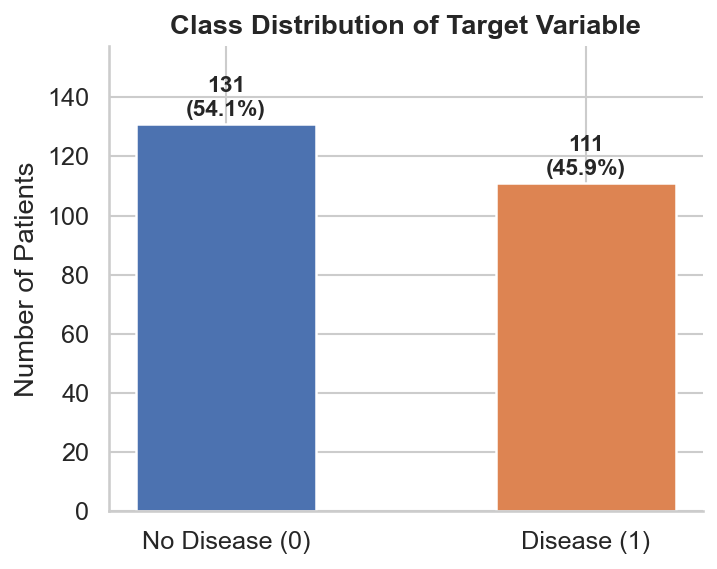
\includegraphics[width=0.6\columnwidth]{figures/fig_class_distribution.png}
    \caption{Class distribution of the target variable. The 1.18:1 ratio motivates the use of stratified folds and class-imbalance-robust metrics throughout the pipeline.}
    \label{fig:class_dist}
\end{figure}

Continuous features showed marked between-class differences for \texttt{thalach} and \texttt{oldpeak} (both Mann-Whitney $p < 0.001$), modest separation for \texttt{age} ($p < 0.001$), and weak separation for \texttt{trestbps} and \texttt{chol} (Fig.~\ref{fig:eda_continuous}). Patients with disease achieved substantially lower maximum exercise heart rates (median $\sim$140 vs $\sim$160 bpm) and higher ST-depression values, consistent with reduced cardiac reserve and exercise-induced ischaemia.

\begin{figure*}[t]
    \centering
    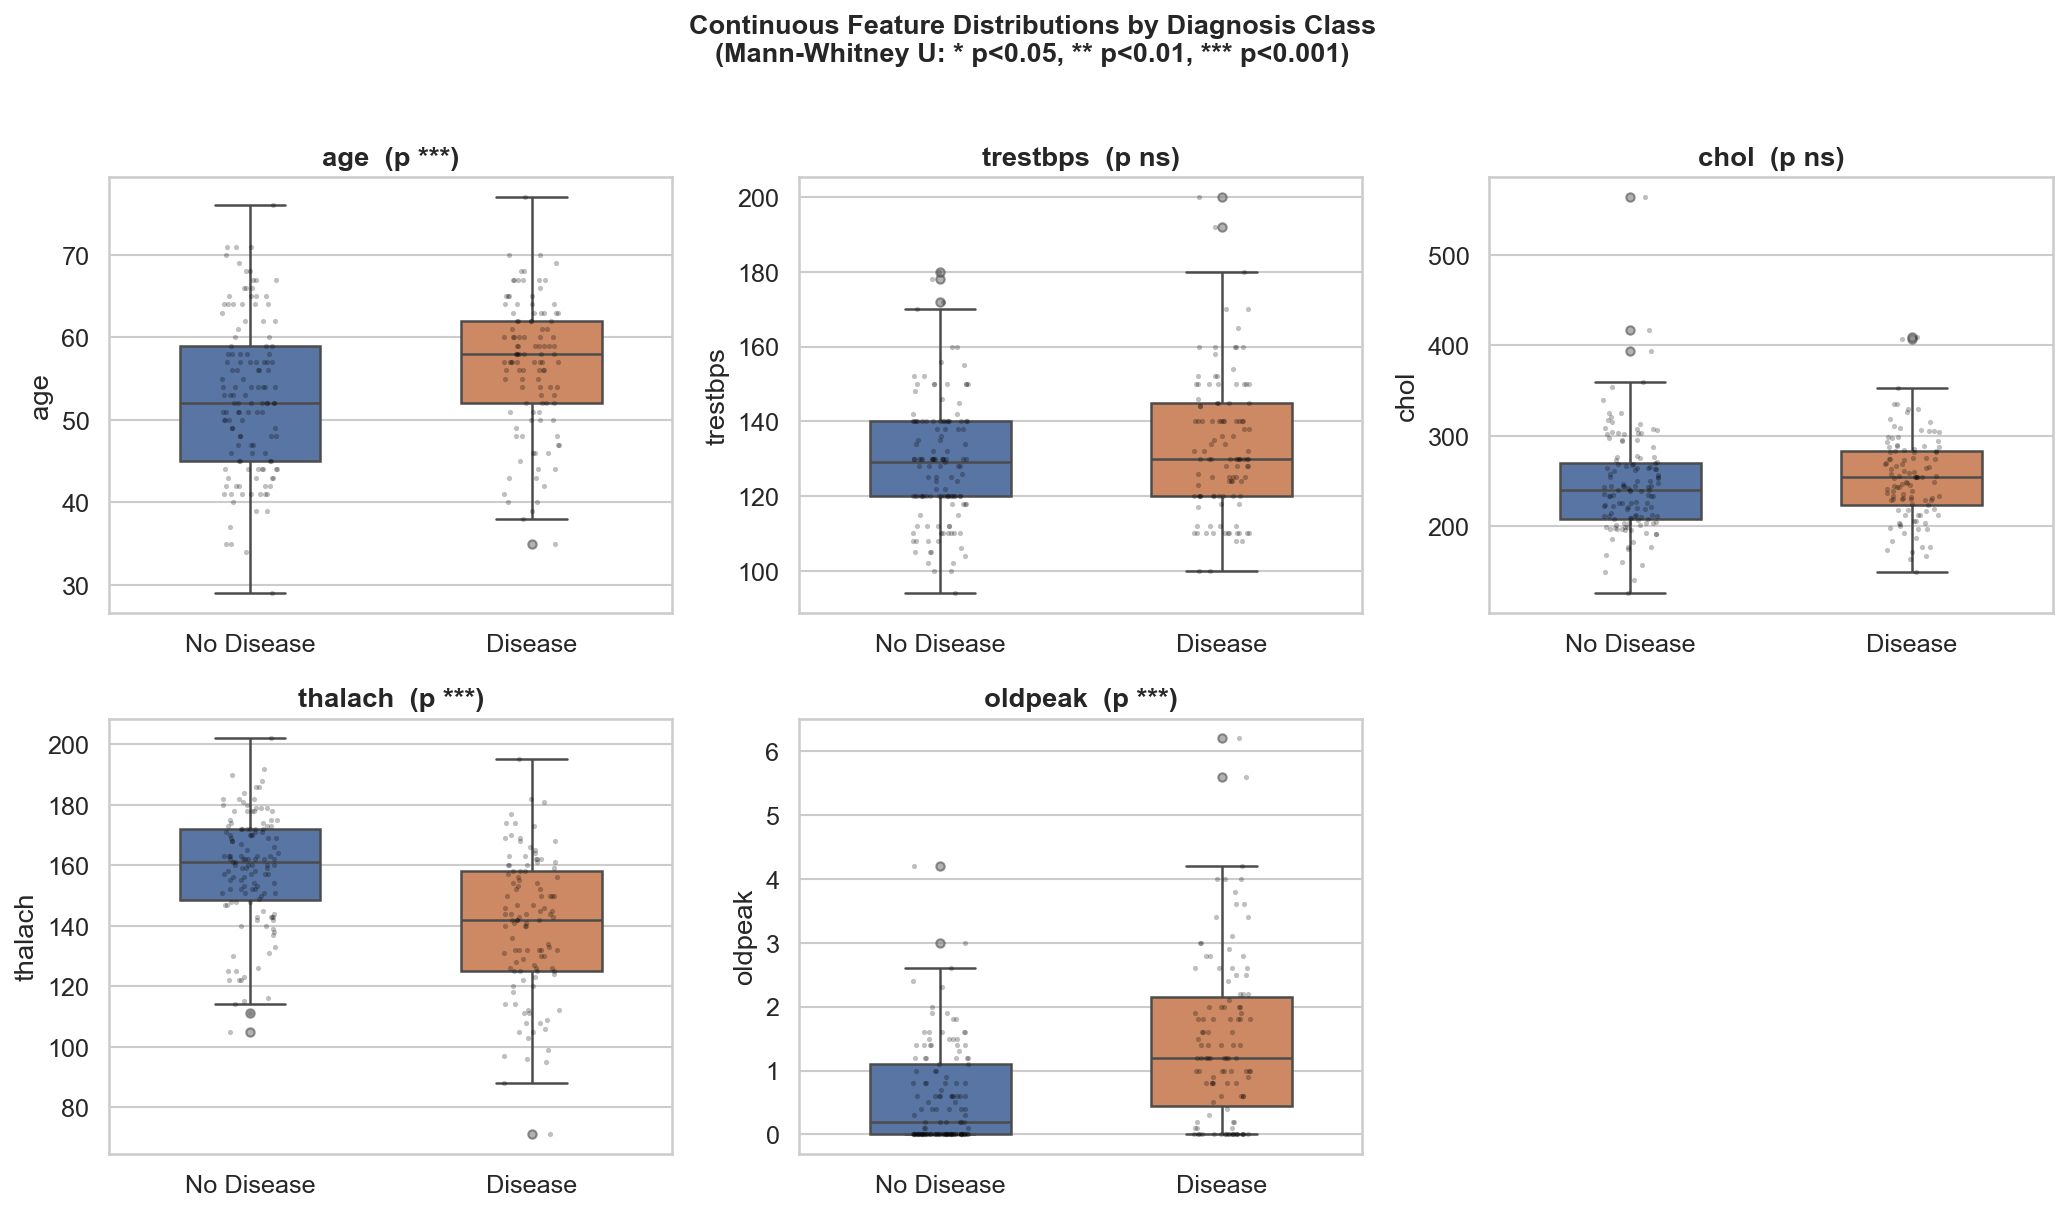
\includegraphics[width=0.85\textwidth]{figures/fig_boxplots_continuous.png}
    \caption{Continuous-feature distributions stratified by diagnosis class. \texttt{thalach} and \texttt{oldpeak} show the strongest separation, both consistent with established markers of coronary ischaemia. Annotated $p$-values are from Mann-Whitney U tests.}
    \label{fig:eda_continuous}
\end{figure*}

The categorical-feature distributions (Fig.~\ref{fig:eda_categorical}) revealed several findings of clinical interest. Asymptomatic chest pain (\texttt{cp}~=~4) was paradoxically the chest-pain category most strongly associated with disease --- a well-established but counter-intuitive pattern attributable to silent ischaemia and the selection bias of a clinical referral cohort. Reversible thallium defects (\texttt{thal}~=~7) were strongly associated with disease, as was a higher number of major vessels affected (\texttt{ca}). Exercise-induced angina (\texttt{exang}) showed a clear discriminative pattern, with $\sim$76\% of patients reporting it having disease versus $\sim$31\% of those without it. Sex showed an epidemiologically expected pattern with higher disease rates in males.

\begin{figure*}[t]
    \centering
    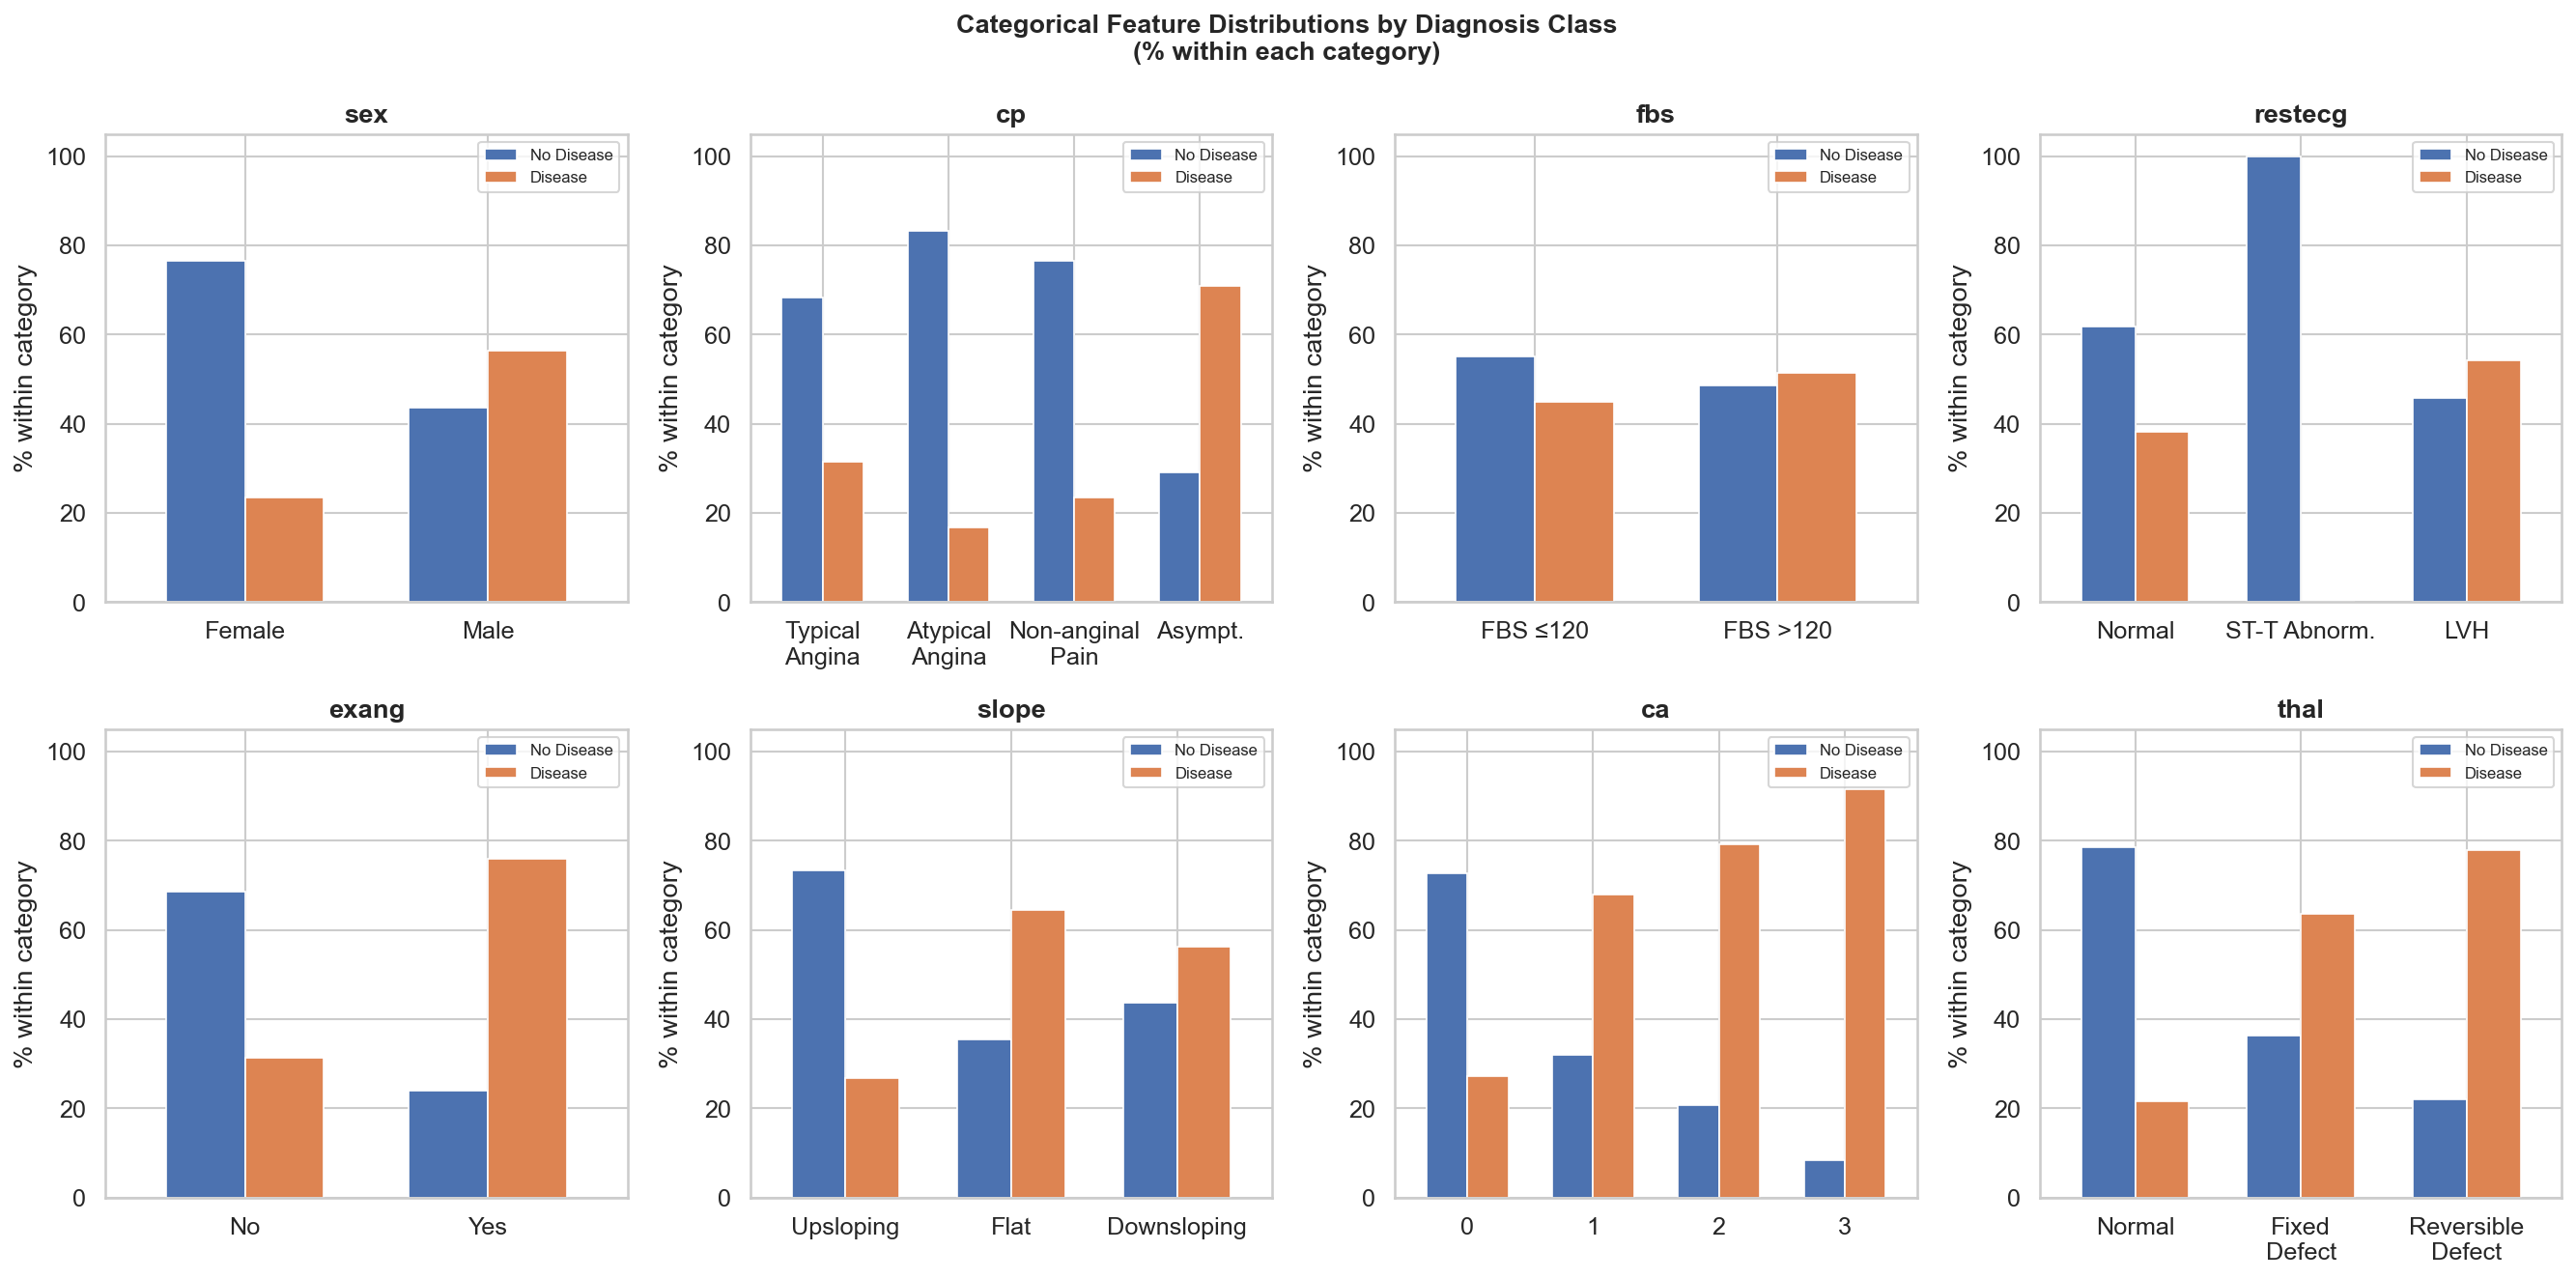
\includegraphics[width=\textwidth]{figures/fig_barplots_categorical.png}
    \caption{Categorical-feature distributions stratified by diagnosis class. The \texttt{cp}, \texttt{thal}, \texttt{ca}, and \texttt{exang} panels each show clear class-discriminative patterns. The \texttt{cp} panel illustrates the silent-ischaemia phenomenon: asymptomatic chest pain (rightmost bar group) is the category most strongly enriched for disease.}
    \label{fig:eda_categorical}
\end{figure*}

The Pearson correlation matrix (Fig.~\ref{fig:eda_corr}) confirmed that no pair of features exhibited high collinearity ($|r| < 0.6$ throughout), and the strongest target correlations were observed for \texttt{thal}, \texttt{ca}, \texttt{exang}, \texttt{thalach}, \texttt{oldpeak}, and \texttt{cp}. Principal component analysis (Fig.~\ref{fig:eda_pca}) showed that the first two principal components explained only 37\% of total variance, with partial class separation visible along PC1. The remaining variance was distributed broadly across components, suggesting that aggressive linear dimensionality reduction would discard meaningful signal --- non-linear classifiers, or linear classifiers operating on the full 13-dimensional feature space, were therefore more appropriate than 2D PCA-based modelling.

\begin{figure}[t]
    \centering
    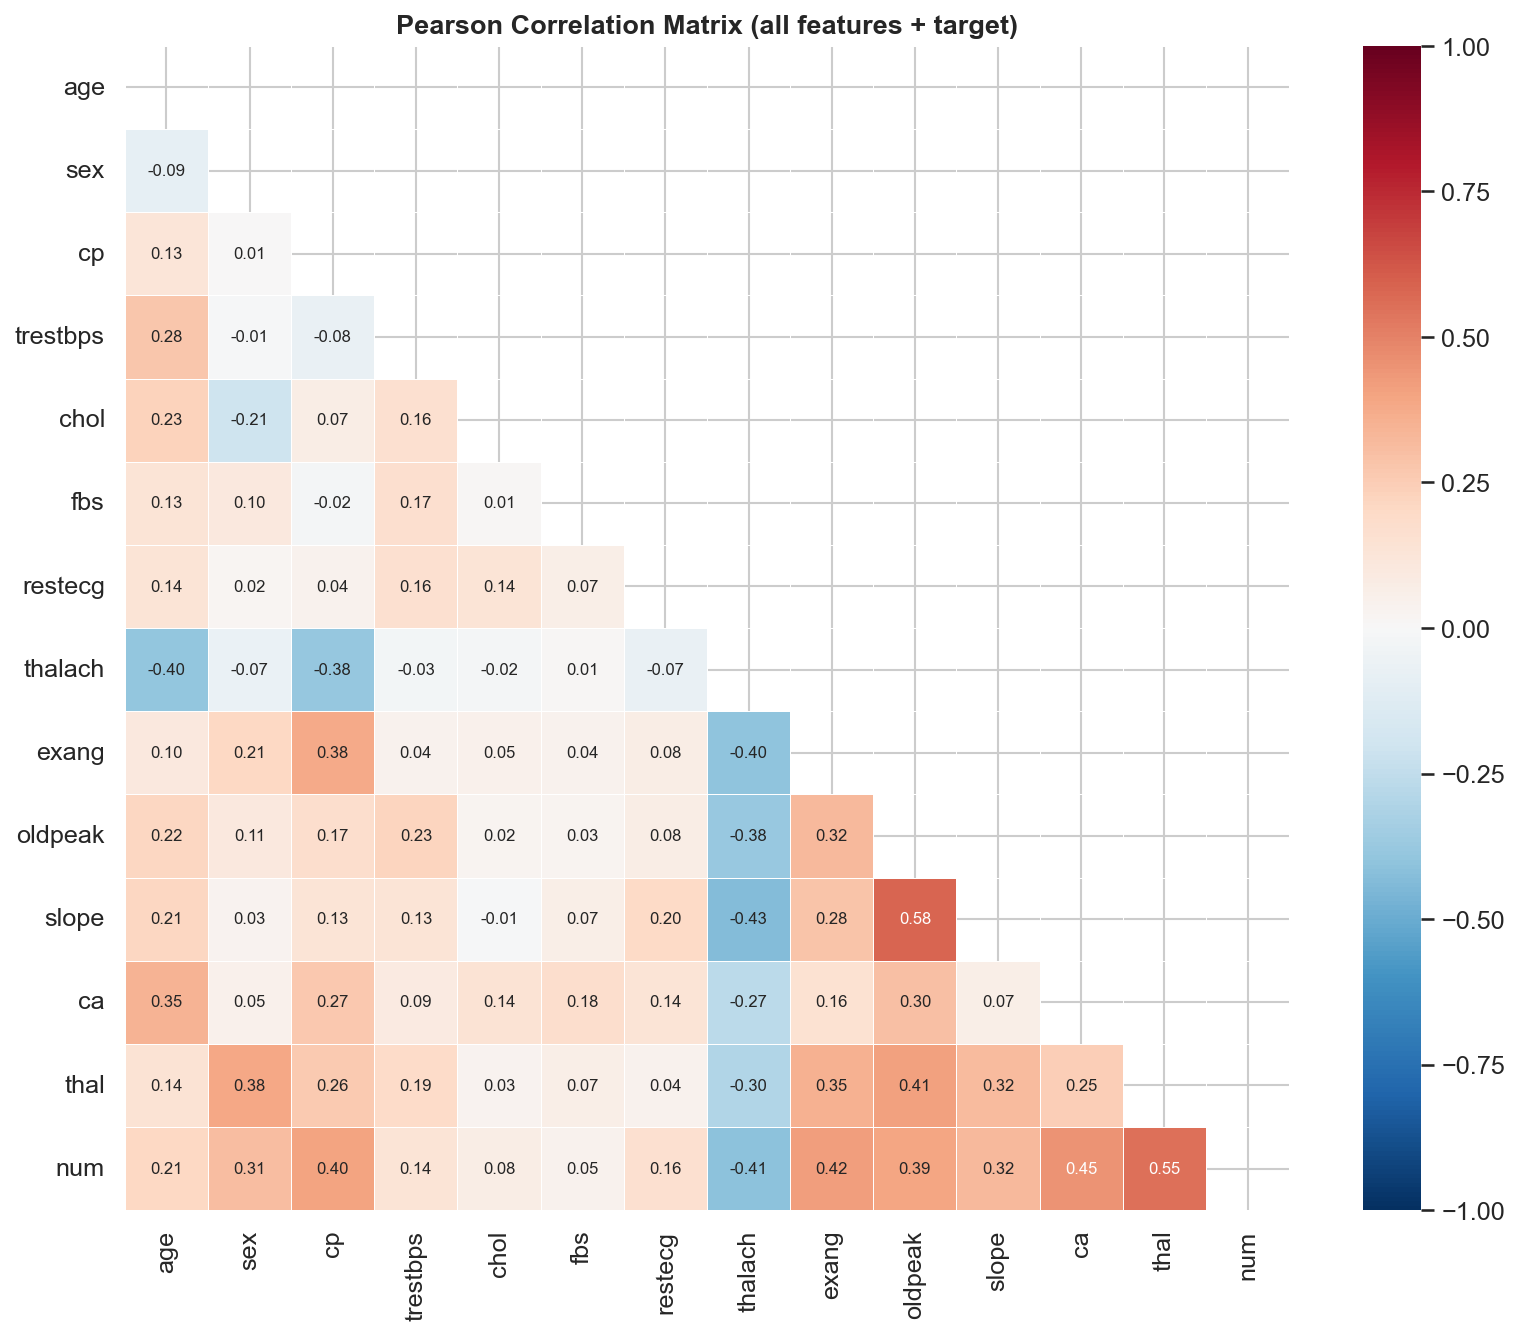
\includegraphics[width=\columnwidth]{figures/fig_correlation_heatmap.png}
    \caption{Pearson correlation matrix. No severe collinearity is observed; the bottom row identifies \texttt{thal} (0.55), \texttt{ca} (0.45), and \texttt{exang} (0.42) as the features most linearly correlated with the target.}
    \label{fig:eda_corr}
\end{figure}

\begin{figure}[t]
    \centering
    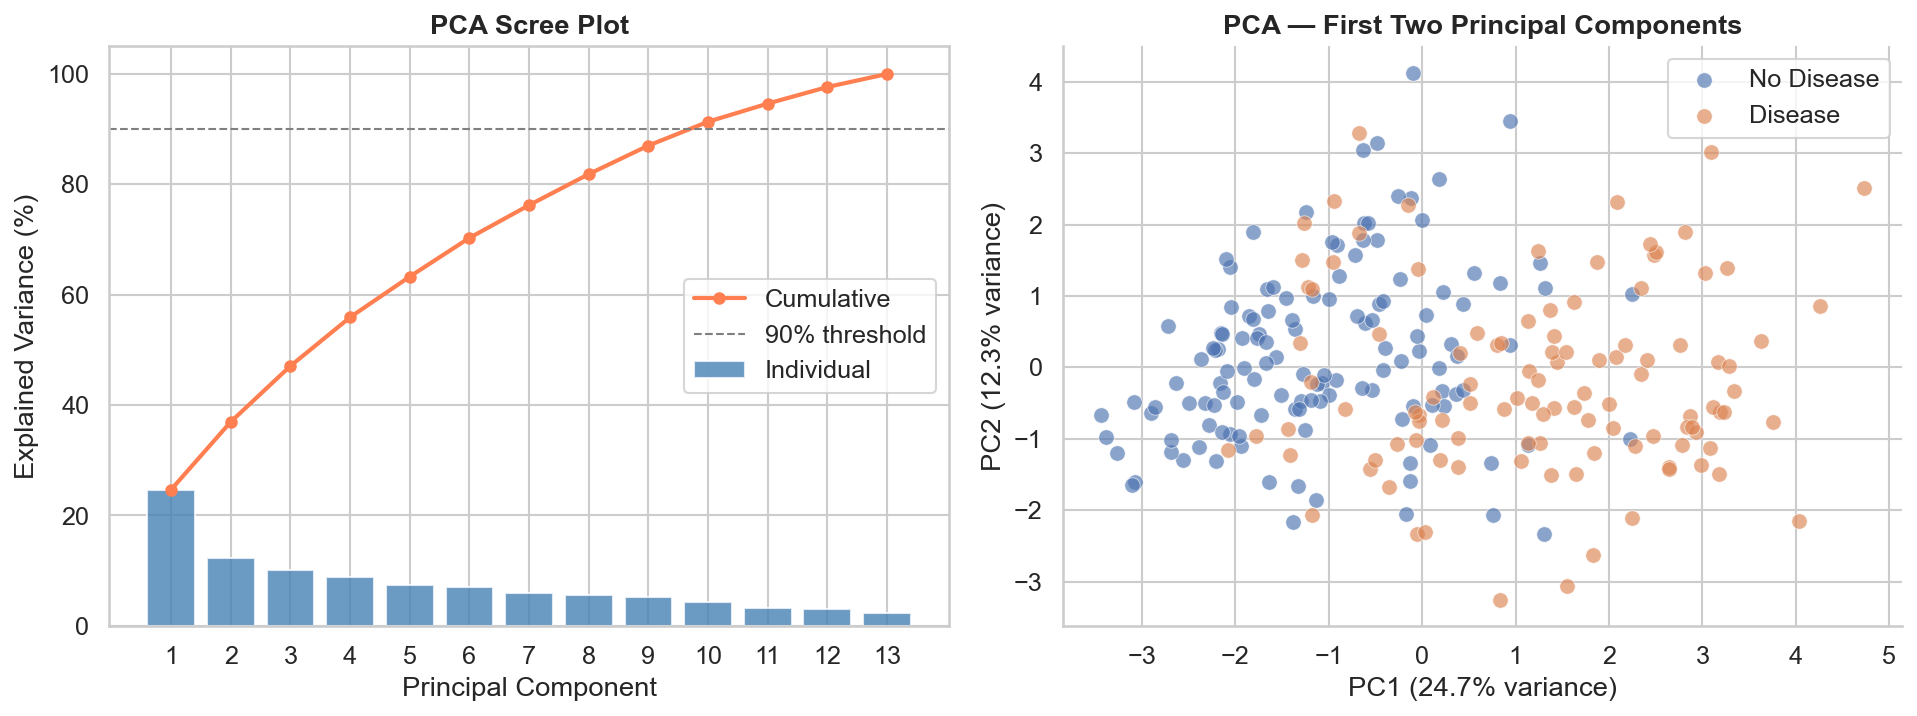
\includegraphics[width=\columnwidth]{figures/fig_pca.png}
    \caption{PCA scree plot (left) and 2D projection on the first two principal components (right). The classes are partially separable along PC1, but the 2D projection retains only 37\% of the variance.}
    \label{fig:eda_pca}
\end{figure}

These EDA findings motivated several preprocessing decisions: mode imputation for the categorical features with missing values, \texttt{StandardScaler} for continuous features only, retention of the \texttt{chol}~=~564~mg/dL outlier as a clinically plausible extreme, and stratified cross-validation throughout. The set of features identified as most informative --- \texttt{cp}, \texttt{thal}, \texttt{ca}, \texttt{thalach}, \texttt{oldpeak}, \texttt{exang} --- would later be revisited in the feature-selection (Section~\ref{sec:results_fs}) and SHAP (Section~\ref{sec:results_shap}) analyses, providing a useful triangulation across the EDA, model-driven feature selection, and post-hoc interpretation.

\subsection{Algorithm Comparison}
\label{sec:results_algocomp}

Table~\ref{tab:algo_baseline} reports per-algorithm performance under default hyperparameters, and Table~\ref{tab:algo_tuned} reports the tuned-rnCV results. Both are summarised as median with 95\% bootstrap CI across the 50 outer-test scores.

\begin{table*}[t]
    \centering
    \small
    \caption{Default-hyperparameter baseline. $R = 10$ iterations of 5-fold stratified CV, no inner loop. Values: median [95\% bootstrap CI].}
    \label{tab:algo_baseline}
    \begin{tabular}{lcccc}
        \toprule
        \textbf{Algorithm} & \textbf{MCC} & \textbf{AUC} & \textbf{PR-AUC} & \textbf{Balanced Acc} \\
        \midrule
        LogisticRegression & 0.640 [0.590, 0.678] & 0.892 [0.876, 0.906] & 0.893 [0.866, 0.912] & 0.815 [0.794, 0.833] \\
        GaussianNB         & 0.642 [0.607, 0.687] & 0.892 [0.878, 0.907] & 0.886 [0.860, 0.901] & 0.817 [0.798, 0.842] \\
        \textbf{LDA}       & \textbf{0.667 [0.628, 0.707]} & \textbf{0.897 [0.881, 0.911]} & \textbf{0.897 [0.874, 0.911]} & \textbf{0.823 [0.809, 0.849]} \\
        RandomForest       & 0.590 [0.577, 0.624] & 0.878 [0.864, 0.901] & 0.876 [0.861, 0.896] & 0.794 [0.779, 0.809] \\
        LightGBM           & 0.553 [0.538, 0.590] & 0.856 [0.837, 0.866] & 0.860 [0.833, 0.871] & 0.775 [0.766, 0.793] \\
        XGBoost            & 0.569 [0.523, 0.593] & 0.859 [0.837, 0.876] & 0.860 [0.844, 0.871] & 0.779 [0.759, 0.796] \\
        CatBoost           & 0.588 [0.550, 0.626] & 0.877 [0.865, 0.892] & 0.875 [0.865, 0.906] & 0.787 [0.774, 0.809] \\
        \bottomrule
    \end{tabular}
\end{table*}

\begin{table*}[t]
    \centering
    \small
    \caption{Tuned-rnCV results. $R = 10$ iterations of 5-fold outer~$\times$~3-fold inner CV, 50 Optuna trials per inner study. Values: median [95\% bootstrap CI].}
    \label{tab:algo_tuned}
    \begin{tabular}{lcccc}
        \toprule
        \textbf{Algorithm} & \textbf{MCC} & \textbf{AUC} & \textbf{PR-AUC} & \textbf{Balanced Acc} \\
        \midrule
        LogisticRegression & 0.627 [0.594, 0.667] & 0.891 [0.872, 0.907] & 0.896 [0.864, 0.912] & 0.811 [0.790, 0.827] \\
        \textbf{GaussianNB} & \textbf{0.642 [0.607, 0.687]} & 0.892 [0.878, 0.907] & 0.886 [0.860, 0.901] & 0.817 [0.798, 0.842] \\
        \textbf{LDA}       & 0.632 [0.623, 0.669] & \textbf{0.895 [0.879, 0.911]} & \textbf{0.894 [0.875, 0.916]} & 0.815 [0.806, 0.825] \\
        RandomForest       & 0.627 [0.585, 0.673] & 0.887 [0.878, 0.907] & 0.893 [0.873, 0.904] & 0.809 [0.793, 0.825] \\
        LightGBM           & 0.582 [0.524, 0.601] & 0.868 [0.849, 0.888] & 0.869 [0.854, 0.881] & 0.783 [0.758, 0.799] \\
        XGBoost            & 0.628 [0.558, 0.664] & 0.888 [0.860, 0.907] & 0.880 [0.867, 0.903] & 0.799 [0.778, 0.829] \\
        CatBoost           & 0.623 [0.558, 0.670] & 0.892 [0.868, 0.907] & 0.888 [0.871, 0.915] & 0.808 [0.778, 0.831] \\
        \bottomrule
    \end{tabular}
\end{table*}

Several patterns emerge. The default-hyperparameter baseline (Table~\ref{tab:algo_baseline}) places LDA at the top with median MCC 0.667, ahead of GaussianNB (0.642) and LogisticRegression (0.640). The tree-based ensembles --- RF, LightGBM, XGBoost, and CatBoost --- trail behind, with median MCC values of 0.553--0.590. After hyperparameter tuning (Table~\ref{tab:algo_tuned}), the gradient-boosting methods improve substantially in MCC (XGBoost: 0.569 $\to$ 0.628; LightGBM: 0.553 $\to$ 0.582; CatBoost: 0.588 $\to$ 0.623), while the linear and discriminant methods change very little. This pattern is illustrated graphically in Figure~\ref{fig:comp_box}. The asymmetry is intuitive: tree-based methods have larger and more consequential hyperparameter spaces than methods like LDA or GNB, so they benefit more from tuning. The convergence after tuning means the ranking is much closer at the top.

\begin{figure*}[t]
    \centering
    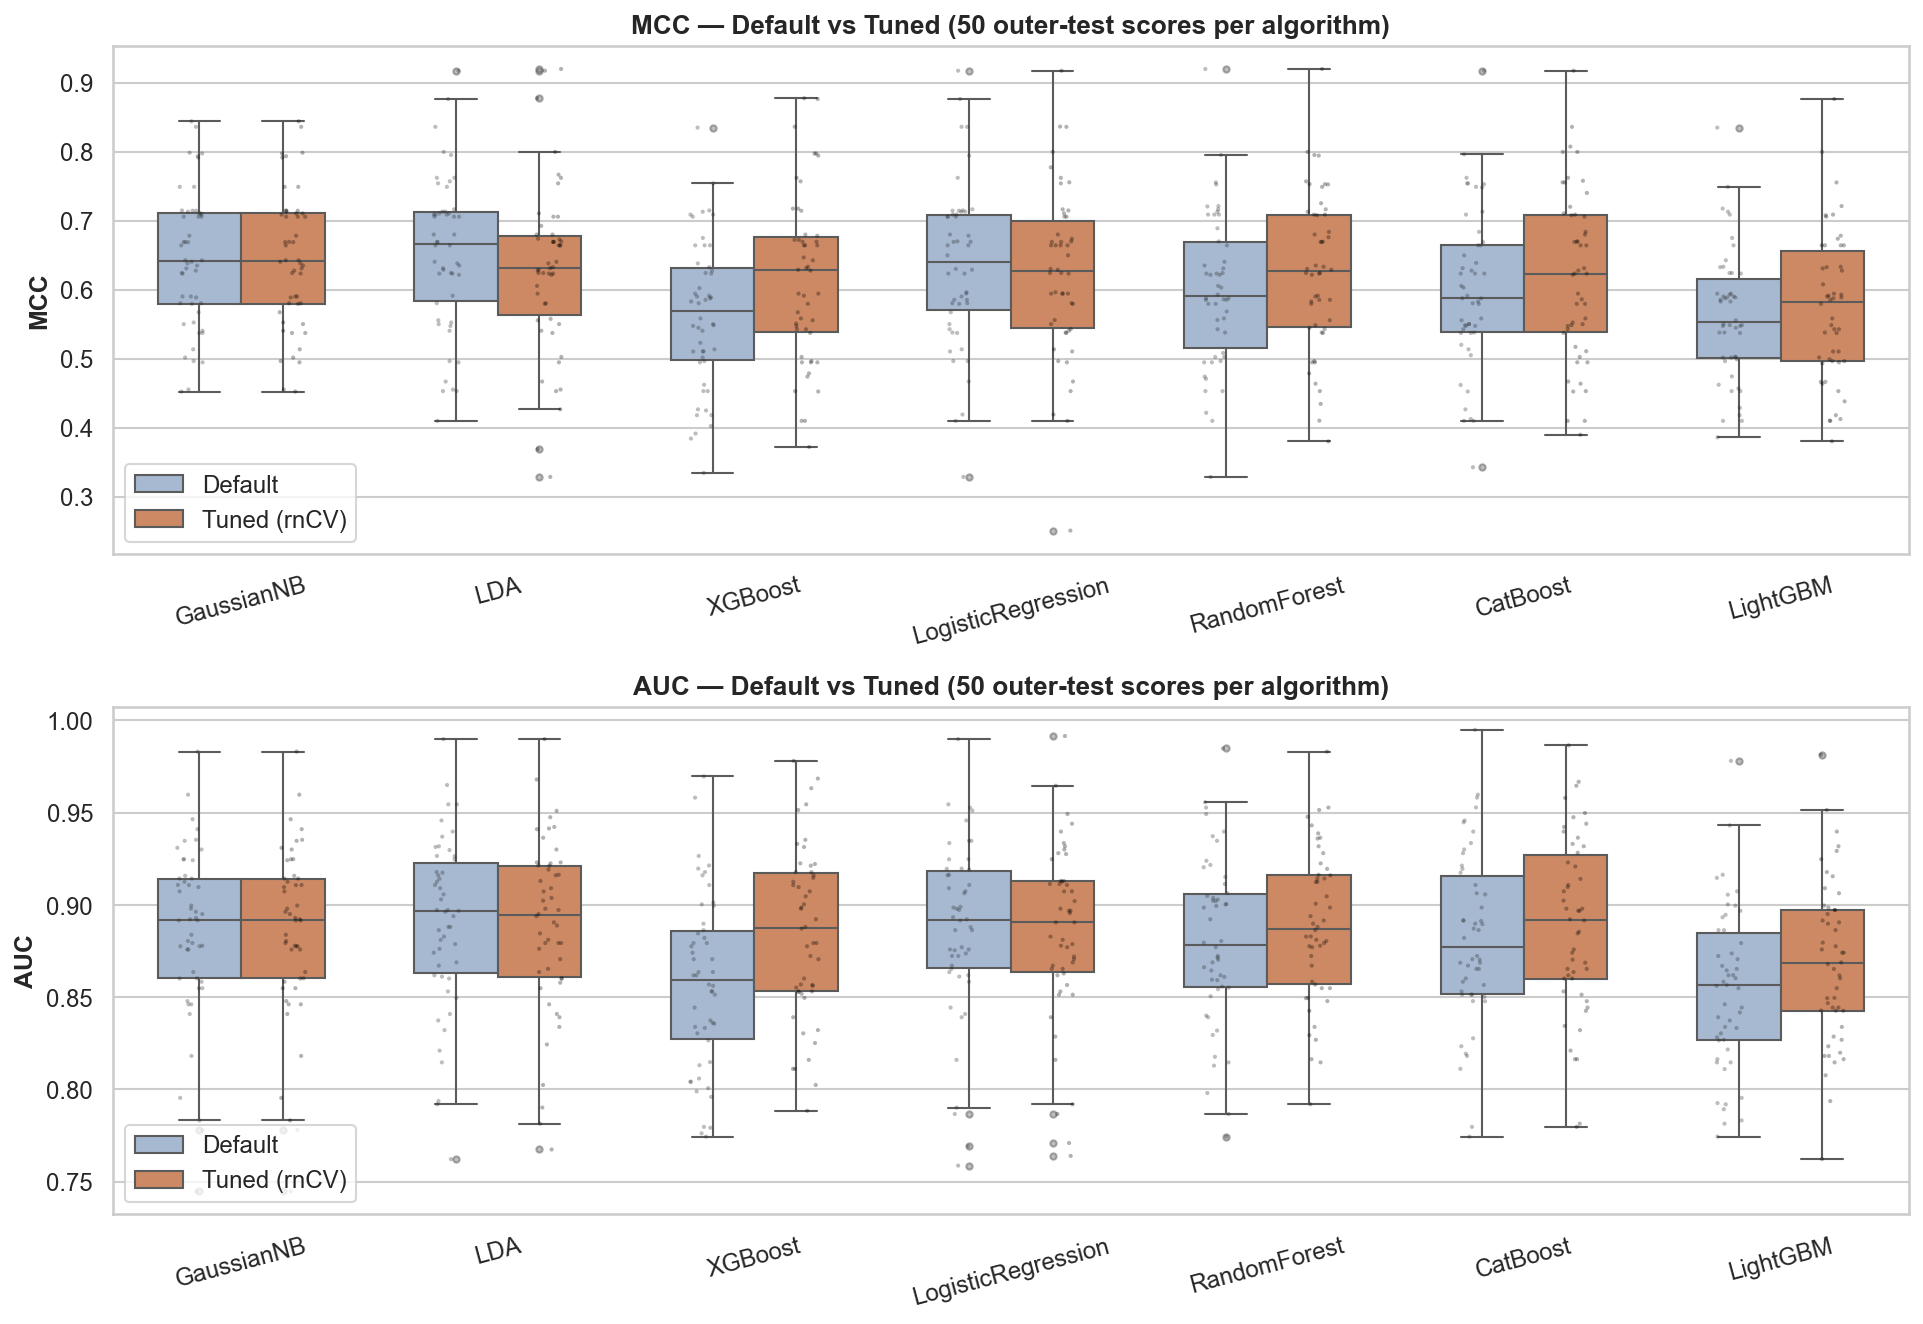
\includegraphics[width=0.95\textwidth]{figures/fig_comparison_boxplots.png}
    \caption{Per-algorithm MCC and AUC distributions across 50 outer-test scores, comparing default and tuned hyperparameters. Tree-based methods benefit visibly from tuning; linear and discriminant methods do not.}
    \label{fig:comp_box}
\end{figure*}

The forest plot of tuned median MCC with 95\% CIs (Fig.~\ref{fig:forest}) shows GaussianNB highest at 0.642, followed by LDA (0.632), XGBoost (0.628), RandomForest (0.627), LogisticRegression (0.627), CatBoost (0.623), and LightGBM (0.582). The CIs of all algorithms except LightGBM overlap one another (Fig.~\ref{fig:ci_overlap}), indicating that on this 242-patient dataset, the top six algorithms are statistically indistinguishable on median MCC alone. LightGBM is the only algorithm whose CI does not overlap LDA's or GaussianNB's, marking it as the only clearly inferior choice.

\begin{figure}[t]
    \centering
    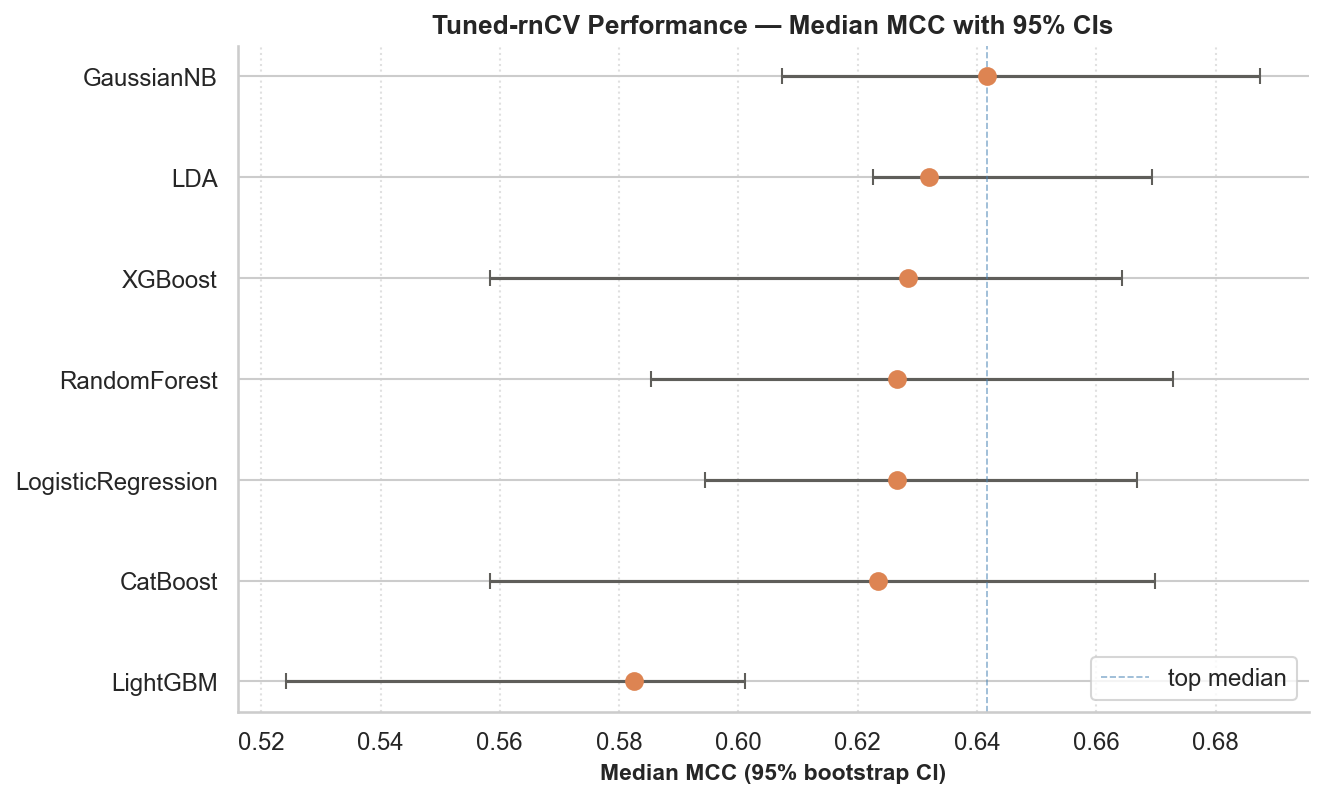
\includegraphics[width=\columnwidth]{figures/fig_mcc_forest.png}
    \caption{Forest plot of tuned-rnCV median MCC with 95\% bootstrap CIs. Six of the seven algorithms have overlapping CIs and are therefore statistically indistinguishable on this metric. LightGBM is the sole outlier.}
    \label{fig:forest}
\end{figure}

\begin{figure}[t]
    \centering
    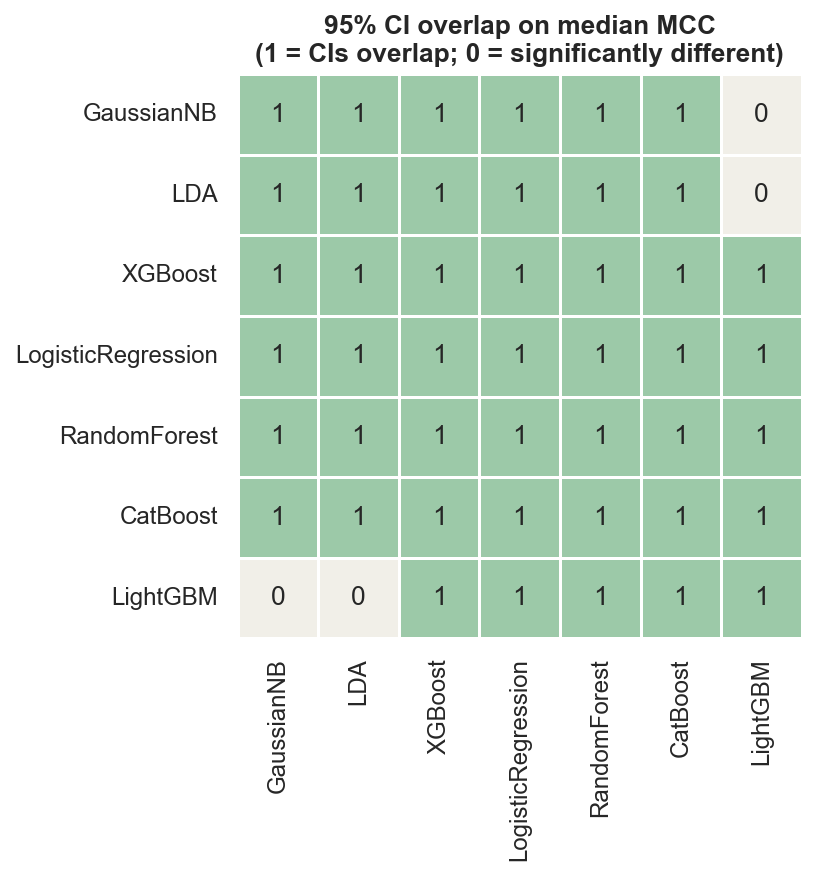
\includegraphics[width=\columnwidth]{figures/fig_ci_overlap.png}
    \caption{Pairwise 95\% CI overlap matrix on median MCC. A value of 1 indicates the two algorithms cannot be distinguished at this confidence level. LightGBM is the only algorithm whose CI does not overlap with both GaussianNB and LDA.}
    \label{fig:ci_overlap}
\end{figure}

Tie-breaking by median AUC and PR-AUC (Fig.~\ref{fig:metric_heatmap}) refines the picture. LDA achieves the highest median AUC at 0.895 and the highest PR-AUC at 0.894, narrowly ahead of GaussianNB (AUC 0.892, PR-AUC 0.886). LDA also achieves the highest specificity (0.885), tied with LogisticRegression and RandomForest. Combining the MCC, AUC, PR-AUC, and specificity rankings, \textbf{LDA was selected as the winning algorithm}. The choice is also defensible on simplicity grounds: among the algorithms statistically tied at the top, LDA has the smallest hyperparameter space and is the most interpretable.

\begin{figure}[t]
    \centering
    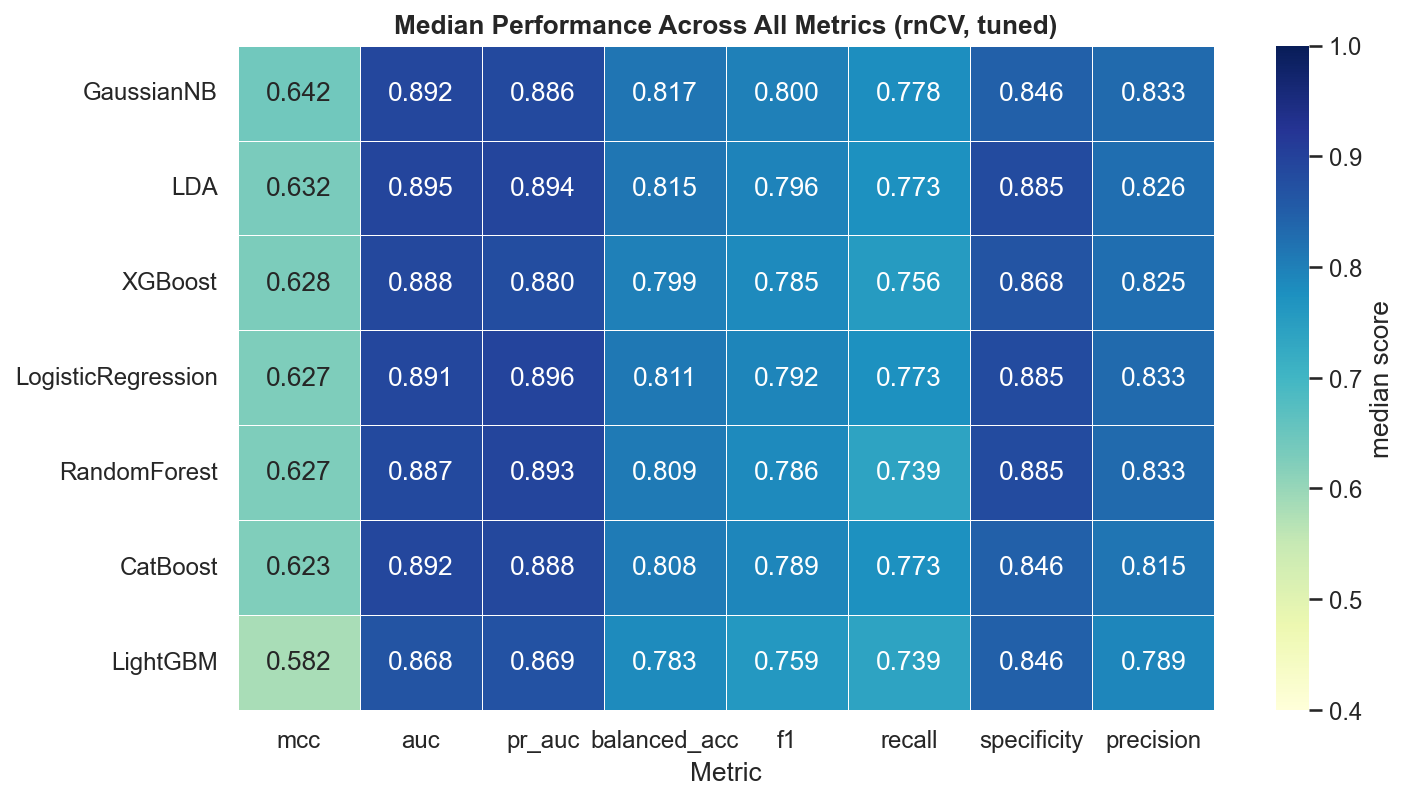
\includegraphics[width=\columnwidth]{figures/fig_metric_heatmap.png}
    \caption{Median performance across all metrics for each algorithm under tuned rnCV. LDA achieves the joint-highest AUC and PR-AUC.}
    \label{fig:metric_heatmap}
\end{figure}

This finding is consistent with the broader literature on small clinical tabular datasets: when $n$ is on the order of a few hundred and the feature count is modest, simple linear and discriminant methods routinely match or exceed the performance of gradient-boosting ensembles. LDA's strong distributional assumptions (Gaussian class-conditionals, shared covariance) act as a powerful regulariser that is helpful when the data are insufficient to constrain a more flexible model. The result is also a useful counter-example to the assumption that gradient-boosting is universally optimal for tabular data.

\subsection{Feature Selection}
\label{sec:results_fs}

The motivating permutation-importance plot (Fig.~\ref{fig:perm_importance}), computed on a single illustrative 80/20 split, ranks the features as \texttt{thal}, \texttt{ca}, \texttt{cp}, \texttt{sex}, \texttt{trestbps}, \texttt{slope}, \texttt{exang}, \texttt{chol}, \texttt{thalach}, \texttt{fbs}, \texttt{restecg}, \texttt{oldpeak}, \texttt{age}. The first three features dominate, separated by a clear gap from the remainder.

\begin{figure}[t]
    \centering
    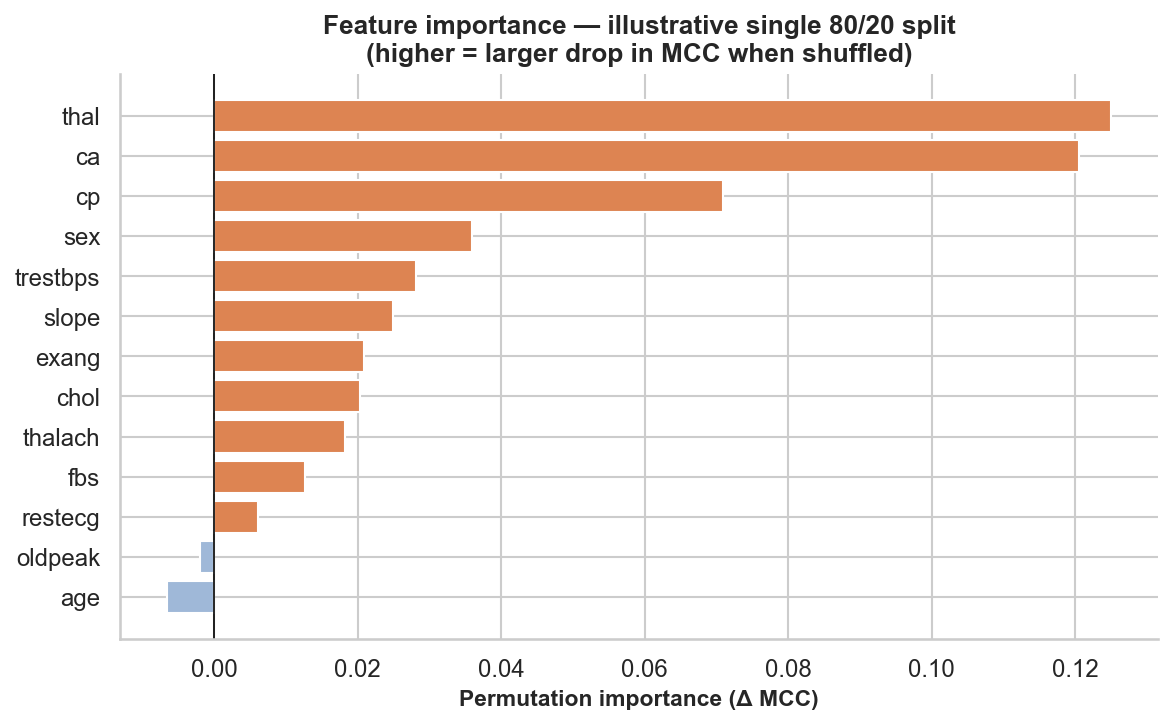
\includegraphics[width=\columnwidth]{figures/fig_perm_importance.png}
    \caption{Illustrative permutation importance on a single 80/20 stratified split. Used here to motivate the choice of method only; actual feature selection was performed independently inside each of the 50 outer folds of the rnCV.}
    \label{fig:perm_importance}
\end{figure}

The performance-vs-$k$ sweep (Fig.~\ref{fig:perf_vs_k}) shows that median MCC rises sharply from $k=3$ ($\sim$0.58) to $k=6$ ($\sim$0.65), peaks in the $k = 7$--$9$ range (median MCC $\sim$0.667 at $k=8$), and then slightly declines for $k \geq 10$. The corresponding AUC curve peaks at $k=9$. This pattern is the textbook bias-variance trade-off: too few features starve the model of signal, while too many introduce noise and increase the effective dimensionality of LDA's covariance estimate beyond what the 242-patient dataset can support. The optimal feature count was therefore set at $k = 8$, achieving median MCC 0.667 and outperforming the full-feature baseline (median MCC 0.632) by $\Delta = +0.035$.

\begin{figure*}[t]
    \centering
    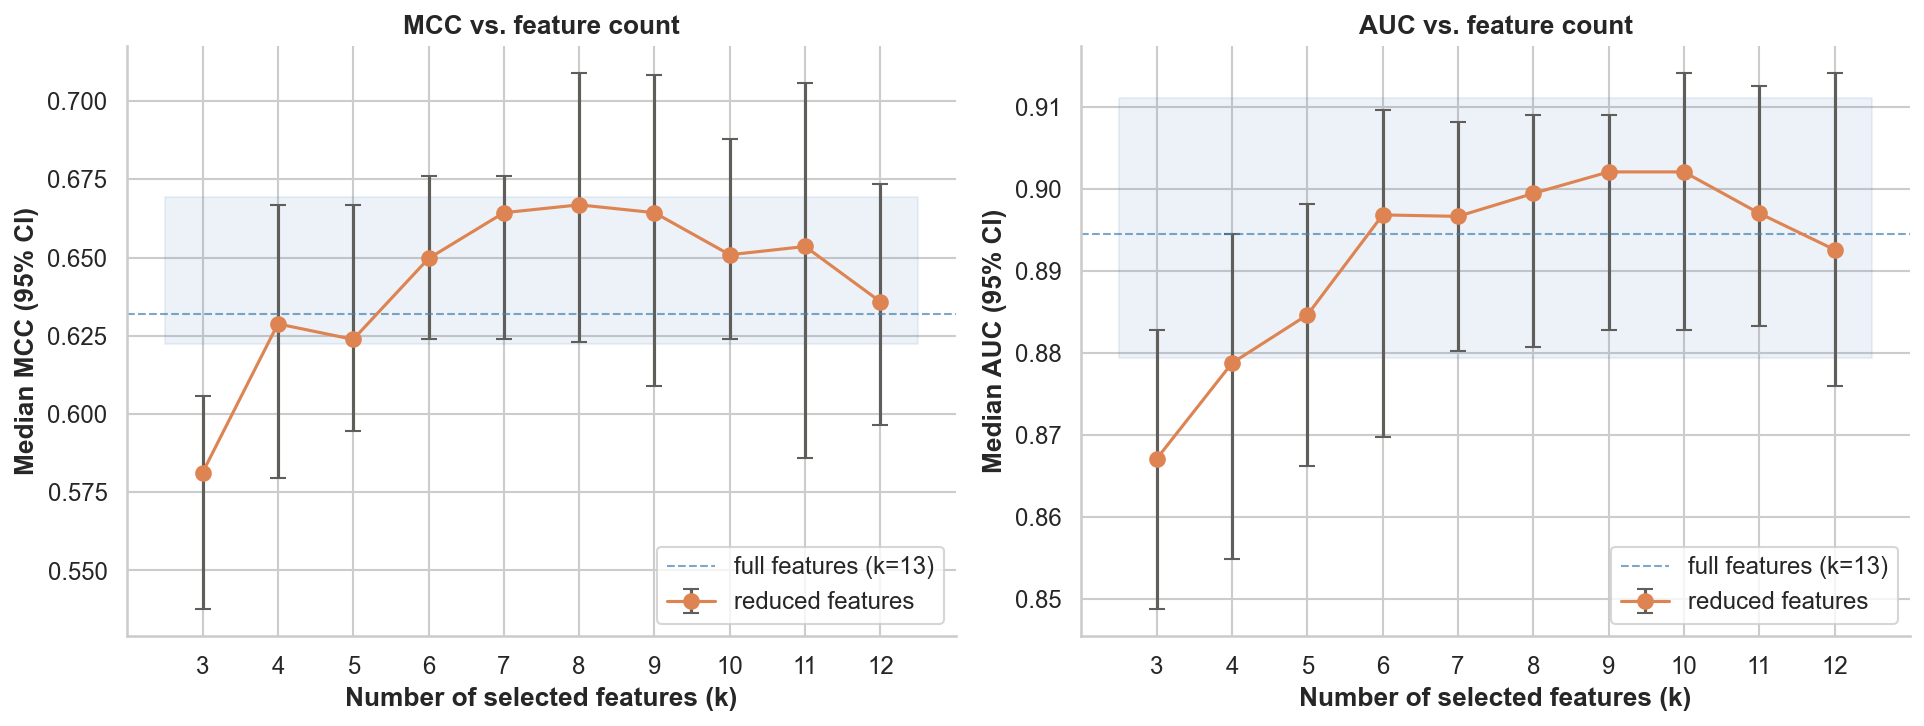
\includegraphics[width=0.95\textwidth]{figures/fig_perf_vs_k.png}
    \caption{Performance versus number of selected features $k$. Median MCC peaks at $k = 8$; AUC peaks at $k = 9$. The full-feature ($k = 13$) baseline is shown as a reference band.}
    \label{fig:perf_vs_k}
\end{figure*}

The per-feature selection frequency at $k = 8$ (Fig.~\ref{fig:sel_freq}) revealed five features selected in $\geq 80\%$ of the 50 outer folds: \texttt{ca} (100\%), \texttt{thal} (100\%), \texttt{sex} (96\%), \texttt{cp} (96\%), and \texttt{exang} (82\%). The remaining three slots rotated between several borderline features (\texttt{thalach} 58\%, \texttt{fbs} 56\%, \texttt{slope} 56\%, \texttt{age} 44\%, \texttt{trestbps} 34\%, \texttt{restecg} 34\%, \texttt{chol} 28\%, \texttt{oldpeak} 16\%), none of which dominated. The selection-frequency distribution is bimodal --- a clear gap separates the five stable features from the remaining candidates --- so the result is robust to moderate variations in the 80\% stability threshold.

\begin{figure}[t]
    \centering
    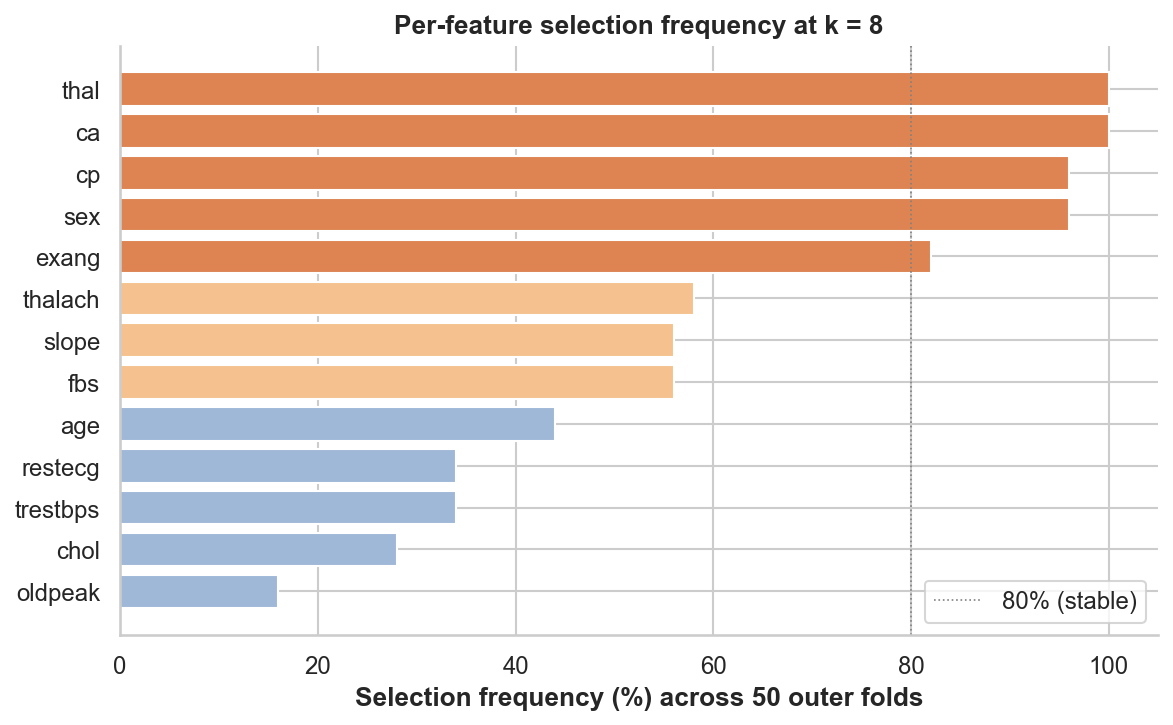
\includegraphics[width=\columnwidth]{figures/fig_selection_frequency.png}
    \caption{Per-feature selection frequency at $k = 8$ across all 50 outer folds (10 repetitions $\times$ 5 outer folds). Five features clear the 80\% stability threshold and constitute the stable feature set used for deployment.}
    \label{fig:sel_freq}
\end{figure}

Two design choices warrant explicit comment. First, the optimal feature \emph{count} ($k=8$) is larger than the stable feature \emph{set} (5 features). The deployed model uses the 5 stable features rather than the 8 selected per fold, prioritising reproducibility and clinical interpretability over a marginal performance gain (the reduced-feature performance comparison in Fig.~\ref{fig:full_vs_red} confirms this is acceptable). Second, the stable feature set comprises only categorical features (\texttt{sex}, \texttt{cp}, \texttt{exang}, \texttt{thal}, \texttt{ca}); none of the continuous features --- \texttt{age}, \texttt{trestbps}, \texttt{chol}, \texttt{thalach}, \texttt{oldpeak} --- entered the stable set despite their visible class-discriminative patterns in the EDA. This is a meaningful clinical finding: the categorical findings of cardiology workup (chest pain type, thallium scan, vessel count, exercise angina, sex) carry sufficient information for LDA to classify reliably without the continuous measurements.

\begin{figure*}[t]
    \centering
    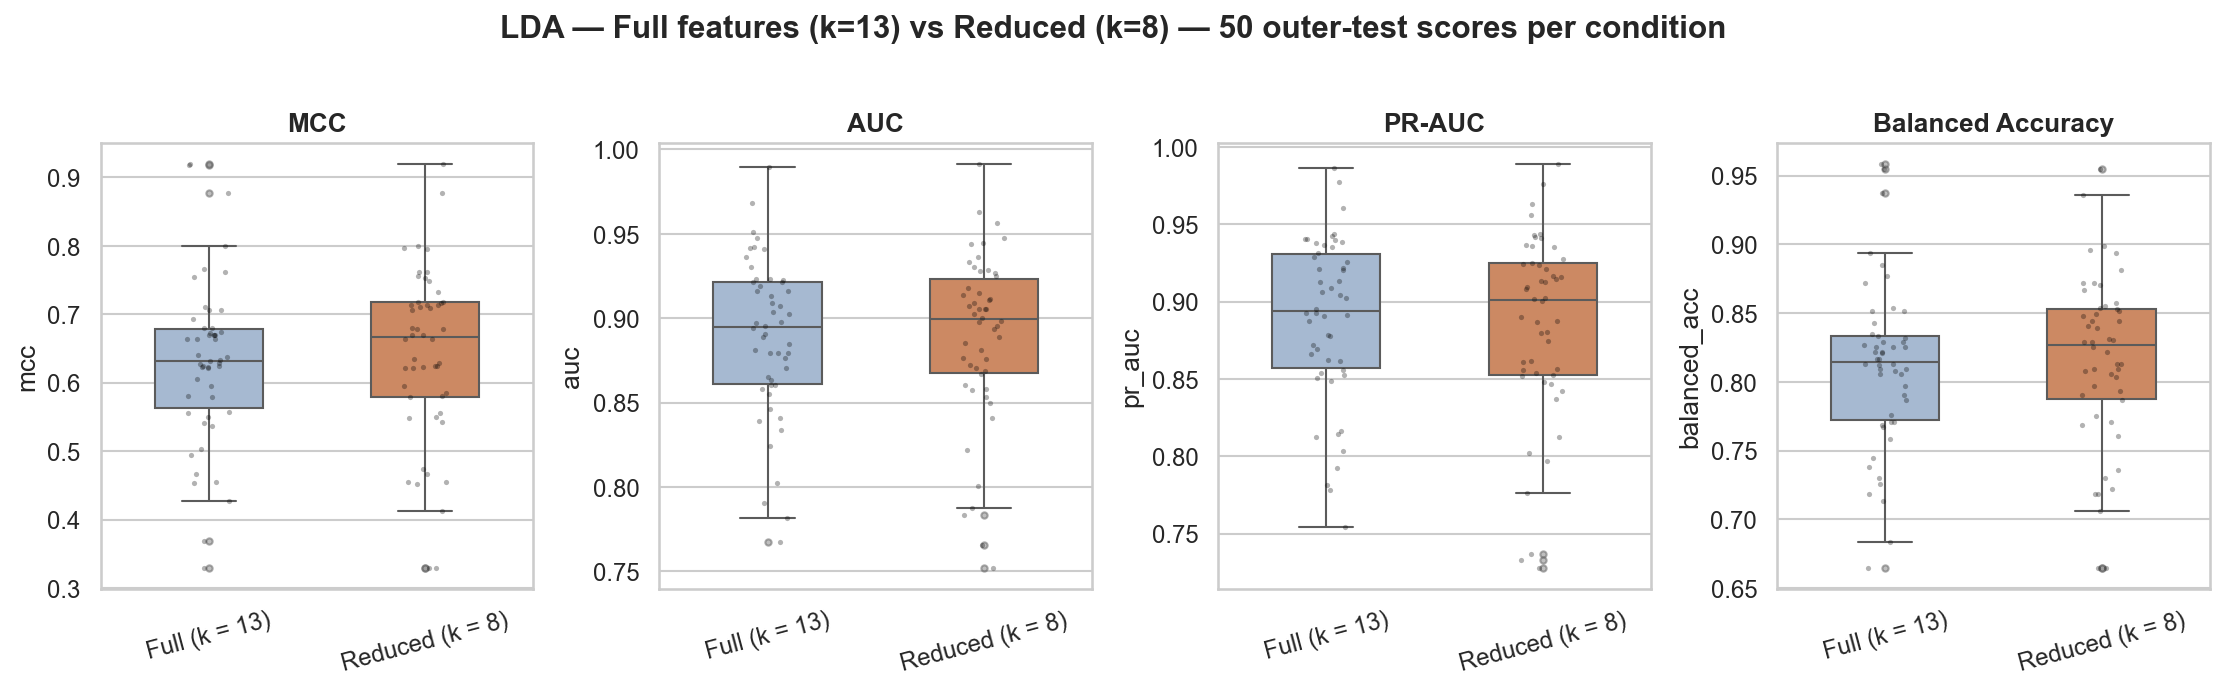
\includegraphics[width=0.95\textwidth]{figures/fig_full_vs_reduced.png}
    \caption{LDA performance on the 13-feature full set versus the $k=8$ reduced set across 50 outer-test scores. Median MCC improves slightly with reduction (0.632 $\to$ 0.667), with all other metrics either improving or holding constant (Table~\ref{tab:full_vs_reduced}).}
    \label{fig:full_vs_red}
\end{figure*}

\begin{table*}[t]
    \centering
    \small
    \caption{LDA — full features ($k=13$) versus reduced ($k=8$). Median [95\% bootstrap CI].}
    \label{tab:full_vs_reduced}
    \begin{tabular}{lcccc}
        \toprule
        \textbf{Condition} & \textbf{MCC} & \textbf{AUC} & \textbf{PR-AUC} & \textbf{Balanced Acc} \\
        \midrule
        Full ($k=13$)   & 0.632 [0.623, 0.669] & 0.895 [0.879, 0.911] & 0.894 [0.875, 0.916] & 0.815 [0.806, 0.825] \\
        Reduced ($k=8$) & 0.667 [0.623, 0.709] & 0.899 [0.881, 0.909] & 0.901 [0.871, 0.914] & 0.827 [0.808, 0.844] \\
        \bottomrule
    \end{tabular}
\end{table*}

The features selected stably converge with the EDA findings (Section~\ref{sec:eda}) on \texttt{cp}, \texttt{thal}, \texttt{ca}, and \texttt{exang} as the most informative variables, with \texttt{sex} also entering the stable set. The agreement between data-driven feature selection and prior clinical knowledge supports the view that the model is exploiting genuine clinical signal rather than dataset artefacts.

\subsection{Final Model and SHAP Interpretation}
\label{sec:results_shap}

A single 5-fold CV with Optuna (50 trials) on the entire dataset using the 5 stable features selected the final hyperparameters \texttt{solver}~=~\texttt{eigen} and \texttt{shrinkage}~=~0.006, achieving a 5-fold mean MCC of 0.680. The chosen \texttt{shrinkage} is essentially zero --- a meaningful finding in itself: with 5 features and 242 patients, the data are sufficient to estimate the LDA covariance reliably without regularisation. If \texttt{shrinkage} had landed near 1.0 it would have signalled insufficient samples per parameter. The 5-fold mean MCC (0.680) is slightly higher than the rnCV estimate (0.632) because the latter uses smaller training folds; the rnCV value remains the appropriate honest estimate of generalisation performance.

The complete deployment pipeline (\texttt{FeatureSubsetSelector} $\to$ \texttt{ColumnTransformer} $\to$ LDA) was fitted on all 242 patients and serialised to \texttt{models/final\_model.pkl}. A reload-and-predict sanity check on raw 13-column input confirmed the artefact functions correctly in a fresh state, addressing the deployability requirement of the assignment.

The SHAP global feature-importance ranking (Fig.~\ref{fig:shap_bar}) places \texttt{thal} clearly first (mean $|\text{SHAP}| \approx 0.19$), followed by \texttt{ca} ($\approx 0.12$), \texttt{exang} ($\approx 0.08$), \texttt{cp} ($\approx 0.08$), and \texttt{sex} ($\approx 0.06$). The fact that \texttt{thal} dominates by a factor of $\sim$1.6 over the next feature reflects its strong direct relationship with disease status in this dataset and is consistent with both the EDA correlations and the stability-selection results.

\begin{figure}[t]
    \centering
    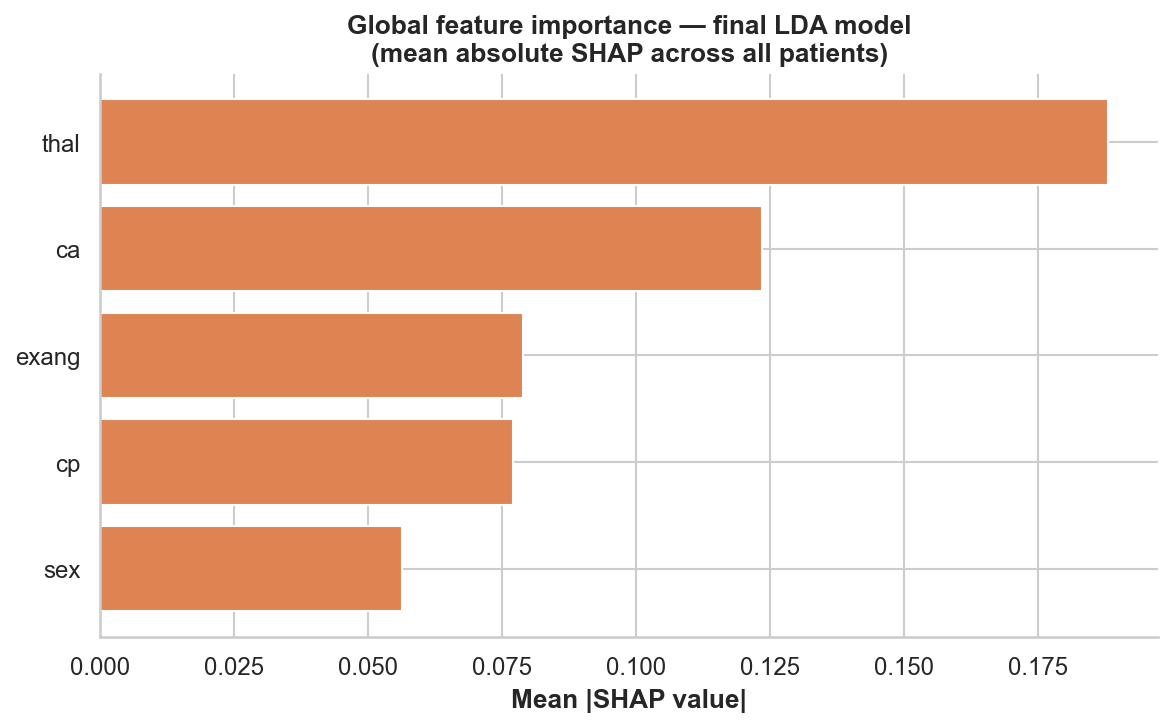
\includegraphics[width=\columnwidth]{figures/fig_shap_bar.png}
    \caption{Global feature importance from SHAP values, computed for the final model on all 242 patients. The thallium scan dominates, followed by vessel count and exercise-induced angina.}
    \label{fig:shap_bar}
\end{figure}

The SHAP summary (beeswarm) plot (Fig.~\ref{fig:shap_summary}) reveals the directional structure of each feature's effect:

\begin{itemize}
    \item \texttt{thal}: bimodal effect. Low values (normal scan, code 3) cluster around SHAP $-0.18$; high values (reversible defect, code 7) cluster around $+0.20$. This is the strongest and most clinically intuitive pattern.
    \item \texttt{ca}: gradient effect. Zero affected vessels push toward no-disease (SHAP $\approx -0.12$); higher vessel counts push progressively toward disease, with some patients reaching SHAP $\approx +0.5$ --- the largest single-feature effect in the dataset.
    \item \texttt{exang}: binary effect, as expected. Presence of exercise-induced angina pushes positively (SHAP $\approx +0.10$); absence pushes weakly negative.
    \item \texttt{cp}: gradient effect with the silent-ischaemia signature. Low \texttt{cp} codes (typical/atypical angina, codes 1--2) push toward no-disease; high codes (asymptomatic, code 4) push toward disease.
    \item \texttt{sex}: binary effect. Females (\texttt{sex}~=~0) push slightly toward no-disease; males (\texttt{sex}~=~1) push slightly toward disease.
\end{itemize}

\begin{figure}[t]
    \centering
    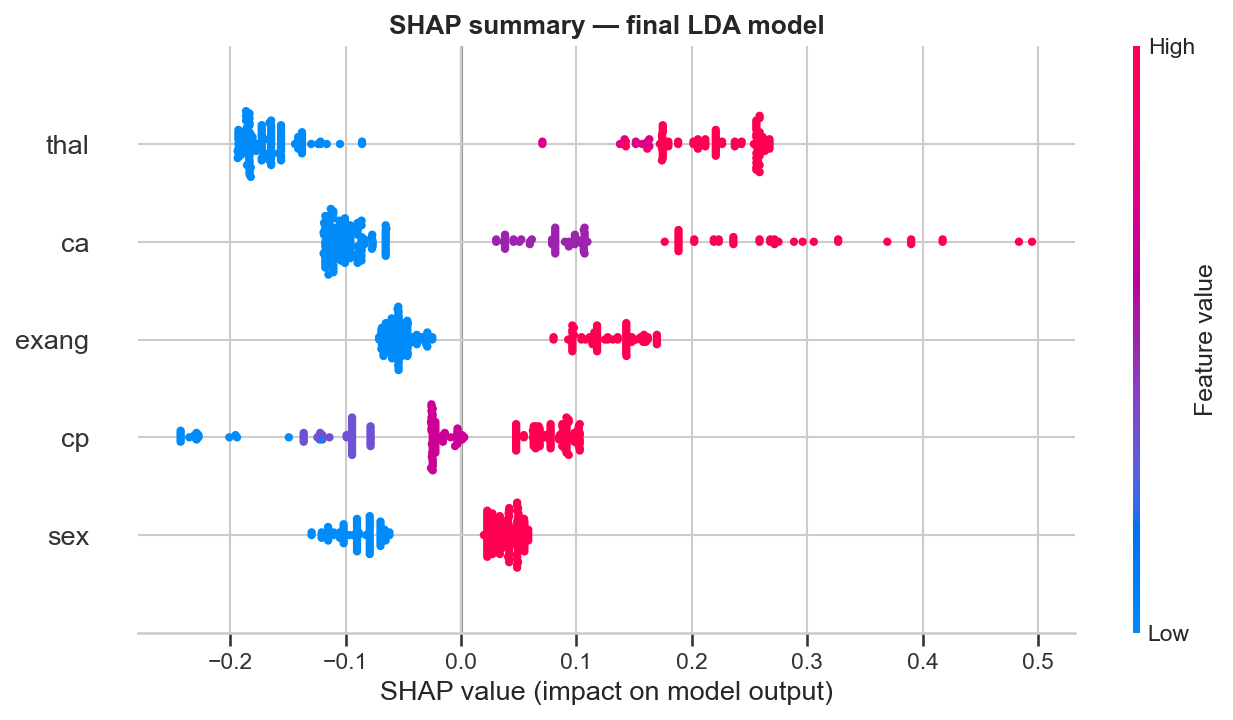
\includegraphics[width=\columnwidth]{figures/fig_shap_summary.png}
    \caption{SHAP summary (beeswarm) plot for the final model. Each point is one patient; horizontal position is the SHAP value; colour encodes feature value (red = high, blue = low). All five features push predictions in clinically expected directions.}
    \label{fig:shap_summary}
\end{figure}

Two individual-prediction explanations are shown in Figure~\ref{fig:waterfalls}. For a correctly predicted disease patient with $P(\text{disease}) = 0.998$, all five features contribute positively, with \texttt{ca}~=~3 (three affected vessels) contributing $+0.26$, \texttt{thal}~=~7 (reversible defect) contributing $+0.14$, and \texttt{exang}~=~1 contributing $+0.08$. For a correctly predicted healthy patient with $P(\text{disease}) = 0.007$, all five features contribute negatively, dominated by \texttt{thal}~=~3 (normal scan) and \texttt{cp}~=~1 (typical angina), each contributing $-0.12$. These waterfall decompositions are the kind of explanation that would support a clinical user in understanding individual predictions, addressing the regulatory transparency expected of any deployed clinical decision-support system.

\begin{figure*}[t]
    \centering
    \begin{subfigure}[b]{0.48\textwidth}
        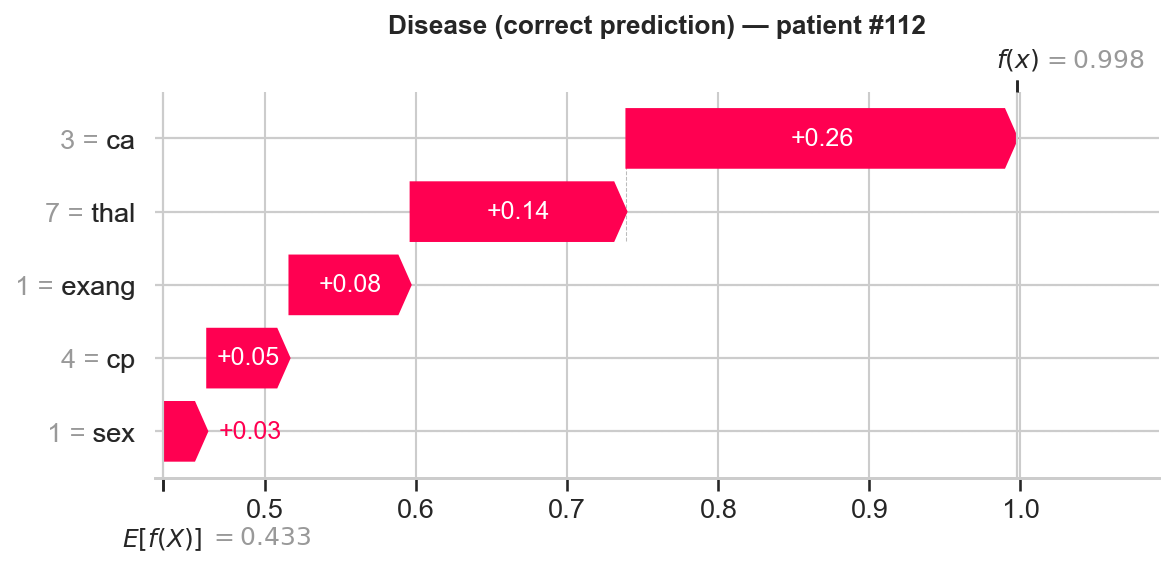
\includegraphics[width=\textwidth]{figures/fig_shap_waterfall_disease.png}
        \caption{Correctly predicted disease patient (\#112), $P = 0.998$.}
    \end{subfigure}\hfill
    \begin{subfigure}[b]{0.48\textwidth}
        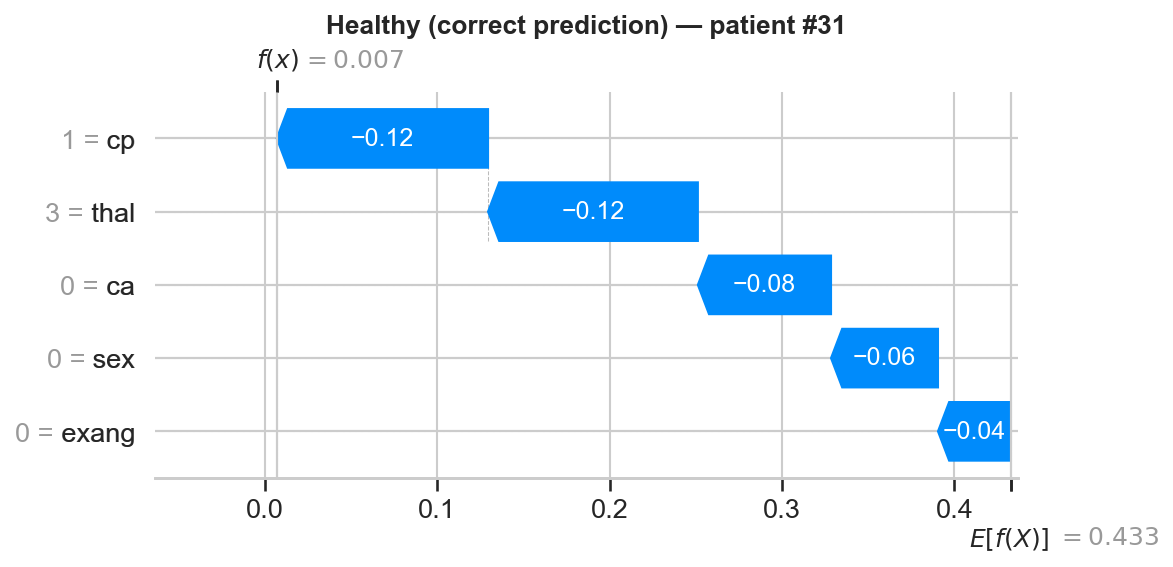
\includegraphics[width=\textwidth]{figures/fig_shap_waterfall_healthy.png}
        \caption{Correctly predicted healthy patient (\#31), $P = 0.007$.}
    \end{subfigure}
    \caption{Individual SHAP waterfall plots. Each bar shows how a single feature value moves the prediction up or down from the model's baseline.}
    \label{fig:waterfalls}
\end{figure*}

The cross-task convergence is the clearest result. The same five features --- \texttt{cp}, \texttt{thal}, \texttt{ca}, \texttt{exang}, \texttt{sex} --- are repeatedly identified as most important by three independent methods: EDA-based statistical analysis (Section~\ref{sec:eda}), permutation-importance feature selection in rnCV outer folds (Section~\ref{sec:results_fs}), and post-hoc SHAP explanations on the final model (this section). This three-way convergence between simple statistical association, model-driven selection, and post-hoc interpretation provides strong evidence that the model has learned genuine clinical signal rather than spurious sample-specific correlations.

\subsection{Bonus Task: Error Analysis}
\label{sec:results_bonus}

The model trained on the 70\% partition (169 patients) and evaluated on the 30\% validation partition (73 patients) achieved 86.3\% accuracy --- 36 true negatives, 27 true positives, 6 false negatives, and 4 false positives (Fig.~\ref{fig:cm}). The validation MCC, AUC, and balanced accuracy were 0.723, 0.920, and 0.859 respectively, all comparable to the rnCV estimates, confirming that the chosen architecture generalises consistently.

\begin{figure}[t]
    \centering
    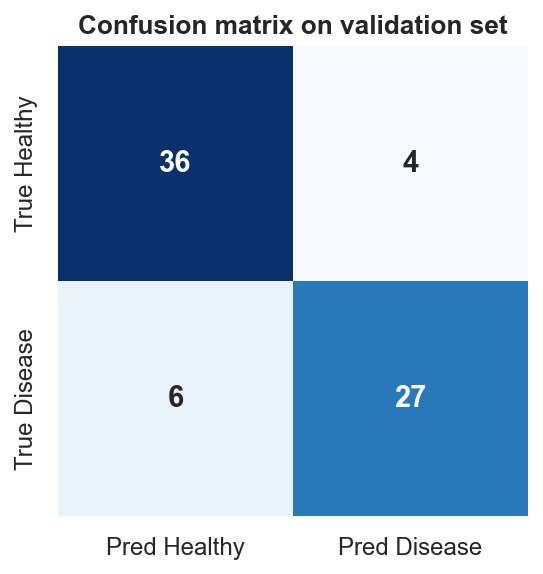
\includegraphics[width=0.55\columnwidth]{figures/fig_confusion_matrix.png}
    \caption{Confusion matrix on the held-out validation set. False negatives outnumber false positives 6:4.}
    \label{fig:cm}
\end{figure}

The ratio of false negatives to false positives (6:4) is clinically relevant: in coronary disease screening, missing disease is more harmful than over-flagging it. This is one motivation for considering a decision threshold below the default 0.5 in deployment, accepting some additional FPs to reduce FNs.

The age comparison (Fig.~\ref{fig:age_cat}) shows that misclassified patients cluster in the 50-60 age band, with no errors observed below age 50 or above 60 in this validation set. The Mann-Whitney comparison of age between correctly and incorrectly classified patients was not statistically significant ($p > 0.05$), but the visual pattern is striking enough to warrant further investigation in larger samples. The effect is more visible in the sex $\times$ age heatmap (Fig.~\ref{fig:err_heatmap}): the 50-60 age band exhibits 23.3\% error rate among males and 20.0\% among females, while the under-50 and over-60 bands exhibit close to zero errors.

\begin{figure*}[t]
    \centering
    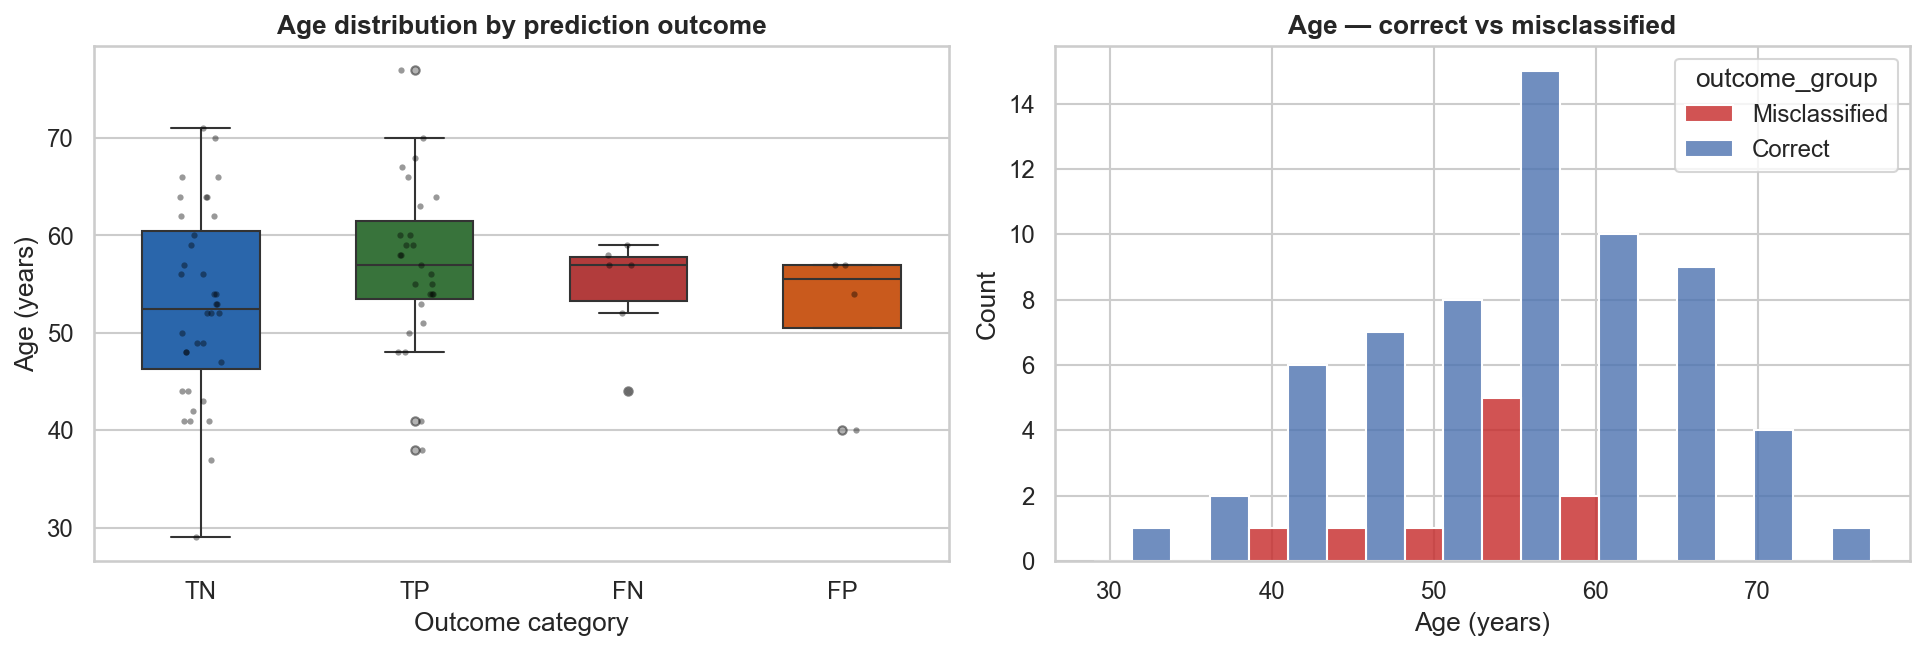
\includegraphics[width=0.85\textwidth]{figures/fig_age_by_category.png}
    \caption{Age distribution by error category (left) and the histogram of correct versus misclassified patients (right). Errors cluster in the 50-60 age band.}
    \label{fig:age_cat}
\end{figure*}

\begin{figure}[t]
    \centering
    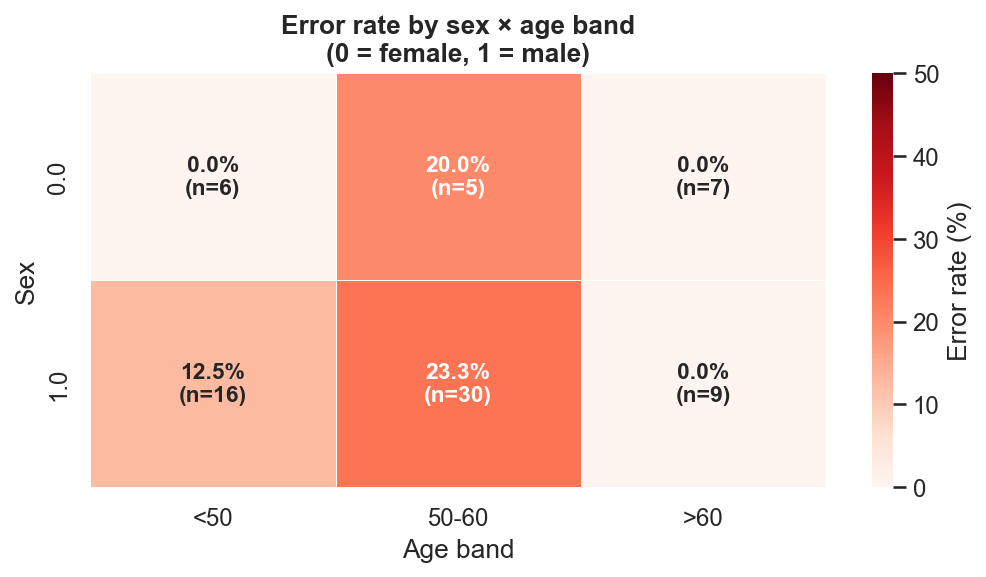
\includegraphics[width=\columnwidth]{figures/fig_error_heatmap.png}
    \caption{Error rate stratified by sex $\times$ age band on the validation set. The 50-60 age band shows the highest error rate ($\sim$20\%) for both sexes; both younger and older patients are classified essentially without error.}
    \label{fig:err_heatmap}
\end{figure}

The most informative finding emerges from the SHAP-by-category analysis (Fig.~\ref{fig:shap_by_cat}). For the model's strongest feature \texttt{thal}, the median SHAP value is $-0.20$ for both TN \emph{and} FN patients, and $+0.28$ for both TP \emph{and} FP patients. In other words, the model's most influential feature pushed FN patients in exactly the same direction as TN patients (toward predicting healthy), and pushed FP patients in exactly the same direction as TP patients (toward predicting disease). The errors occur because \texttt{thal} was \emph{misleading} for those specific patients --- they are diseased patients whose thallium scan was normal, or healthy patients whose thallium scan was abnormal. This is a textbook clinical reality: thallium scans are imperfect proxies for coronary disease, and the model's reliance on this strong but imperfect feature is the dominant source of its errors.

\begin{figure*}[t]
    \centering
    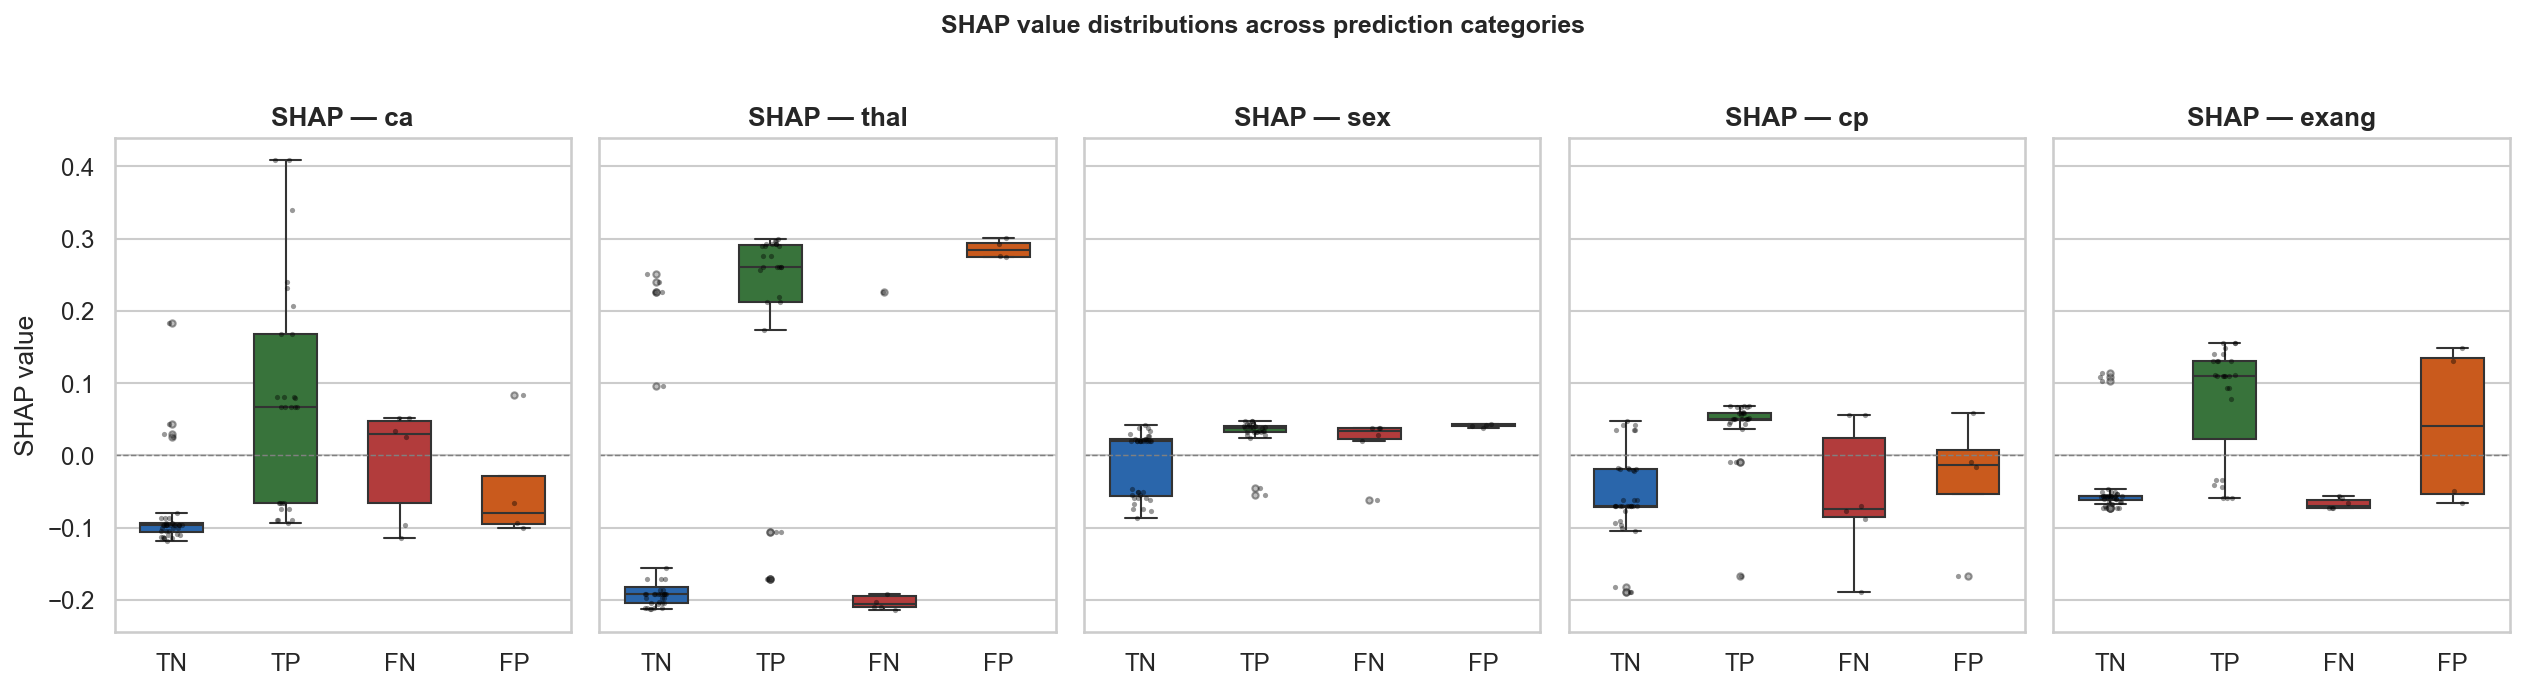
\includegraphics[width=0.95\textwidth]{figures/fig_shap_by_category.png}
    \caption{SHAP value distributions across the four error categories (TN, TP, FN, FP). The \texttt{thal} panel reveals the dominant error mechanism: FN patients have SHAP values nearly identical to TN patients, indicating that the thallium scan was the primary driver of the misclassification.}
    \label{fig:shap_by_cat}
\end{figure*}

The same pattern is visible at the level of raw clinical-feature values (Fig.~\ref{fig:feat_by_cat}), confirming that the SHAP findings reflect a real clinical signal rather than an artefact of how the model uses the features. FN patients exhibit \texttt{thal}~=~3 (normal scan) and low \texttt{ca} values (median $\sim 1$ vessel), almost indistinguishable from TN patients --- yet they were truly diseased. FP patients exhibit \texttt{thal}~=~7 (reversible defect) and \texttt{cp}~=~3--4 (non-anginal or asymptomatic), patterns that closely resemble TP patients --- yet they were healthy. This double confirmation, at both the SHAP-contribution level and the raw-feature level, makes a clear point: the model is not malfunctioning; it is correctly extrapolating from feature values that happen to be misleading for the specific patient. This is the inherent imperfection of any decision-support model that relies on diagnostic findings which are themselves imperfect proxies for the underlying disease.

\begin{figure*}[t]
    \centering
    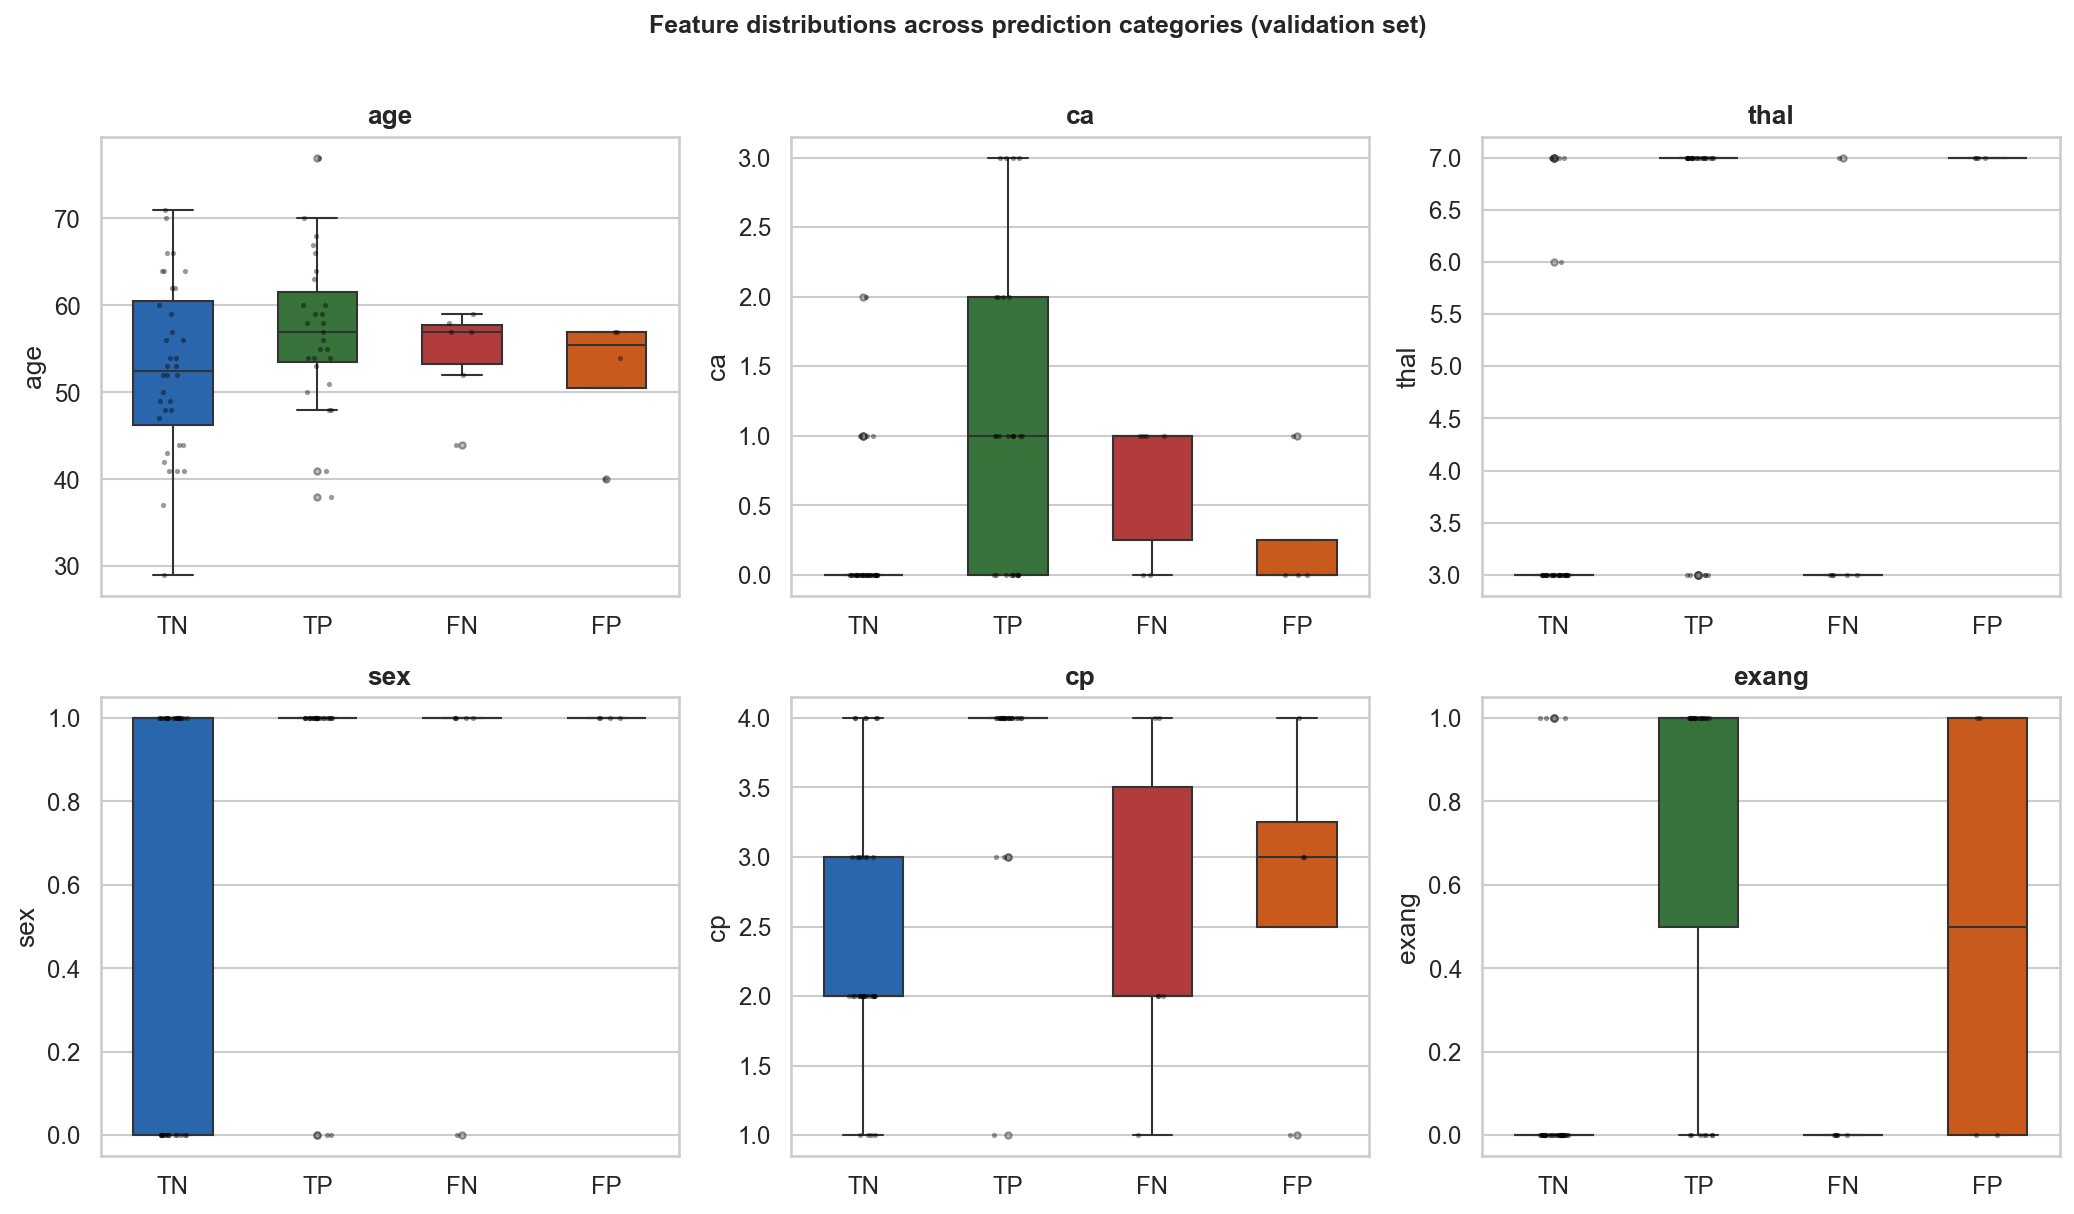
\includegraphics[width=0.95\textwidth]{figures/fig_features_by_category.png}
    \caption{Raw clinical-feature distributions across the four error categories (TN, TP, FN, FP) on the validation set. FN patients (red) closely resemble TN patients (blue) on the dominant features \texttt{thal} and \texttt{ca} despite being truly diseased; FP patients (orange) closely resemble TP patients (green) on the same features despite being healthy. This explains the SHAP-by-category pattern (Fig.~\ref{fig:shap_by_cat}) at the level of underlying clinical findings.}
    \label{fig:feat_by_cat}
\end{figure*}

Figure~\ref{fig:proba_cat} confirms that the errors cluster near (but not exactly at) the decision boundary: the FN group has predicted probabilities centred around 0.22 with maximum 0.33, while the FP group has probabilities centred around 0.74 with minimum 0.58. None of the errors occurred at very high or very low probabilities, suggesting a probability-based triage strategy may be useful: patients with predicted probability between 0.30 and 0.70 should perhaps be routed to additional clinical review rather than acted on by the model alone.

\begin{figure}[t]
    \centering
    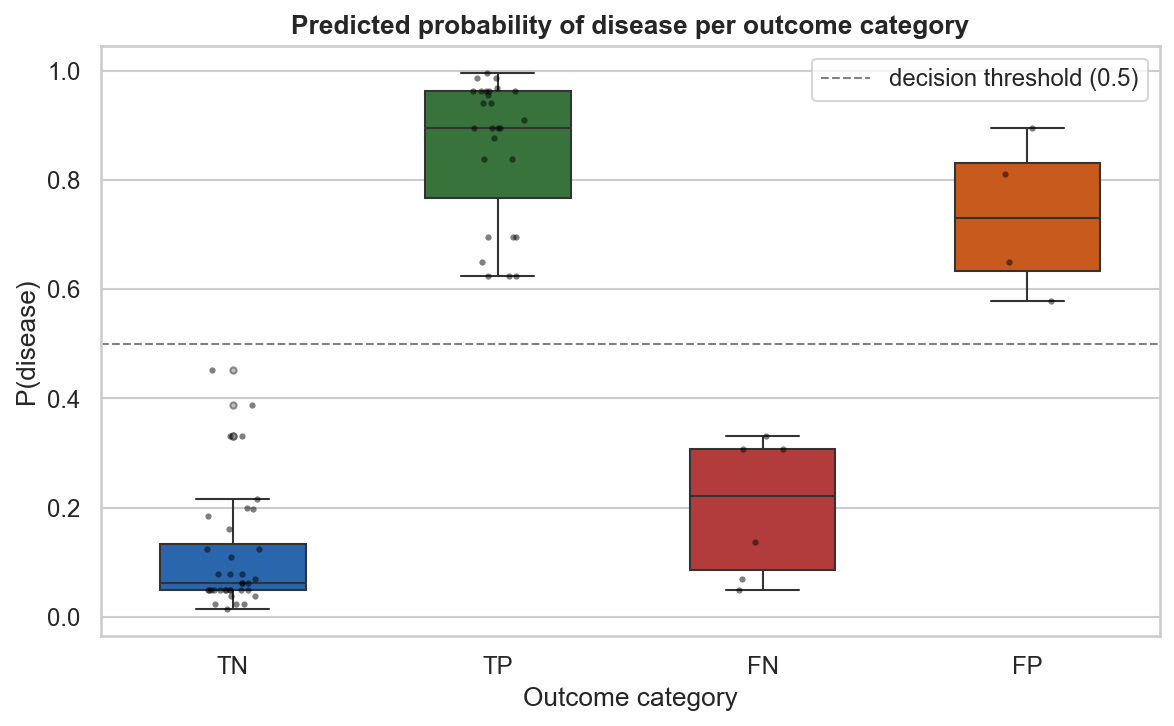
\includegraphics[width=\columnwidth]{figures/fig_proba_by_category.png}
    \caption{Predicted probability of disease per outcome category. Errors occupy the moderate-probability region (FN: 0.05--0.33; FP: 0.58--0.89), suggesting a clinical triage strategy.}
    \label{fig:proba_cat}
\end{figure}

\paragraph{Clinician-oriented summary.}
The model bases its decisions on five clinical findings drawn from routine cardiology workup: thallium scan, number of major vessels affected on fluoroscopy, chest pain type, exercise-induced angina, and patient sex. Each contributes in a clinically expected direction. The model is highly reliable when these findings concord (TP and TN groups have well-separated predicted probabilities). Errors occur when the dominant feature, the thallium scan, is misleading for an individual patient: a normal thallium result in a diseased patient, or an abnormal result in a healthy one. Patients with predicted probabilities in the moderate range (0.30--0.70) are those the model itself indicates as ambiguous, and should be subject to additional clinical review. Errors in the present validation set were concentrated in the 50-60 age band and absent in younger and older patients. A bias toward false negatives over false positives (6:4 ratio) suggests that any deployment should consider lowering the decision threshold below 0.5 to favour sensitivity. The model is suitable as a clinical decision-support aid but should not be used as a stand-alone diagnostic tool.
